\documentclass[twocolumn]{svjour3}

\smartqed  % flush right qed marks, e.g. at end of proof

\usepackage{graphicx}
\usepackage{amsmath}
\usepackage{amssymb}
\usepackage{amsfonts}
\usepackage{textcomp}
%\usepackage{latexsym}
%\usepackage{mathptmx}
\usepackage[utf8]{inputenc}

\tolerance=9999
\pretolerance=\tolerance
\emergencystretch=30pt


\journalname{The Visual Computer}

\begin{document}



\title{Towards a General Model for Virtual Worlds Generation}


% [G. L\'opez, R. Molina \& J. Gallego]
\author{Gabriel L\'opez-Garc\'ia \and
        Rafael Molina-Carmona \and
        Javier Gallego-S\'anchez}

\institute{ Grupo de Inform\'atica Industrial e Inteligencia Artificial\\
            Universidad de Alicante, Ap.99, E-03080, Alicante, Spain\\
            Tel.: +34 96 590 3400\\
            Fax:  +34 96 590 3902\\
            \email{\{glopez, rmolina, ajgallego\}@dccia.ua.es} }

\maketitle



\begin{abstract}
One of the most important problems in Virtual Reality (VR) is the diversity in displays and interaction devices. Moreover, the heterogeneity in rendering, physics and artificial intelligence engines causes the inexistence of a comprehensive and coherent model which combines all the features of a VR system. A new formal model is proposed to solve these diversity problems.

The proposed model, based on a grammar, integrates the visualization and the interaction with a complete VR system. The world is described as a sequence of ordered primitives, transformations and actors, in a broad sense. Primitives are not just drawing primitives, but actions which operate in a representation system. Transformations are used to change the behaviour of primitives. Actors represent the activities in the virtual world which are carried out through events.

The resulting model separates the activity of the system from the devices that originate it. It has several advantages: devices can be easily replaced or simulated; system components can be reused; and the graphic representation can be different depending on the visual device. In short, this paper proposes a comprehensive, adaptive, reusable and generic model. Finally, a practical example is presented to prove the effectiveness of this model.

\keywords{  Virtual Reality \and
            Virtual Worlds generation \and
            Formal model \and
            Interaction}

\end{abstract}




%___________________________________________________________________________
\section{Introduction
\label{sec:introduction}}
%___________________________________________________________________________

In recent years, the development of Virtual Reality (VR) and graphical systems has been amazing \cite{Sherman2003}.
This progress has contributed to the creation of new ways to analyze and work with information, such
as graphics, animations or simulations. Computer games industry is one of the elements which has
contributed most to the advance of graphical systems and to the emergence of new VR systems \cite{Novak2007}.
However, these developments have opened up new challenges.

One of the most important problems is the wide variety of visual devices (monitors, PDAs, cell
phones, VR goggles), each one with different features. For that reason, it is necessary to develop
adaptive systems which generate the images according to the specific characteristics of the device
(resolution, size, ...).

While the processes of visualization and renderization of images have reached a certain maturity in
the past decades, in the field of interaction a similar evolution has not been produced
\cite{Joshua2004,David2005}. Keyboard and mouse still dominate the world of interactive devices.
High degree-of-freedom input devices are complex to manage, and other possibilities of interaction
are only used in research and graphic art \cite{Joshua2004}. However, there has been tentative
progress in recent years. Wii's input device is a highlight among them \cite{wiiNintendo}.

It is necessary to develop a model which unifies the whole range of devices of interaction and
visualization. For example, the action of moving an object in the virtual world, should not be
connected with the push of a specific button on a mouse, a keyboard, or any other device. Instead,
this diversity of events should be unified in one action: ``move the object'', removing this way
all the specific characteristics of the different devices.

In the development of VR systems, there are three major modules which have had an uneven evolution.
These are the Graphics, the Physics and the Artificial Intelligence (AI) engines \cite{Burdea2003}.
The first one handles the display of data into visual devices. The second one simulates all the
physical processes, providing more coherent actions and visual effects to the virtual world \cite{Wikipedia2007}.
The last one tries to simulate an intelligent and independent behaviour of the actors in the scene.

Multiple tools and solutions to develop these three modules have been proposed (see Section
\ref{sec:background}). However, there are no unified criteria to deal with the different
development challenges. Some common points have been used to define certain structural designs, but
there is no study about the connections between the different modules.

This paper presents a new model which integrates the diversity of the VR systems and the
aforementioned modules (Graphics, Physics and AI engines). The major goal is to
separate the scene definition from the hardware-dependent characteristics of the system devices. It
uses a grammar definition which integrates activities, visualitation and interaction with users.

The following section describes the state of the art of VR systems and the related definition
languages. Section \ref{sec:objectives} shows the main objectives to achieve. Section
\ref{sec:model} defines the proposed model, and Section \ref{sec:case_study} presents a case study.
Finally, the conclusions and the lines for future work are shown.



%___________________________________________________________________________
\section{Background
\label{sec:background}}
%___________________________________________________________________________

A VR system can be considered to be composed of three main modules: rendering system, physics
engine and AI system. It is also necessary to use a definition language to model the graphical
environment and its behavior in the system. Next, the background of these modules are reviewed
briefly.

There are two main libraries which are used to develop components of graphics engines: Direct3D
\cite{DirectX} and OpenGL \cite{OpenGL}. Both libraries are defined as a layer between the
application and the graphics card. Different systems which try to unify these two APIs
(\textit{Aplication Program Interfaces}) into a single interface have appeared. This is the case of
OGRE \cite{OGRE} and VTK \cite{VTK}. There are also libraries which are used to manage the
interactive hardware. Two examples are SDL \cite{SDL} and DirectX \cite{DirectX}. In general, they
have similar features, but SDL is open source and cross-platform.

There are a large variety of tools which implement physics engines \cite{Seugling2006}, such as Working Model
\cite{WModel} (used mainly in the area of education to perform simulations), Newton Game
Dynamics \cite{NGDynamics}, Physics Abstraction Layer (PAL) \cite{PAL} (it is an open source and
cross-platform API for physical simulation), Open Dynamics Engine (ODE) \cite{ODE} (it is an
implementation of a part of the PAL specifications), and so on.  There are many other API among
the proprietary software, such as PhysX \cite{Physx} (developed by NVidia
and used in the PlayStation 3) and Havok \cite{Havok} (it belongs to the company Havok and it is
implemented for Windows, MacOS, Linux, Xbox 360, Wii, Playstation3 and PlayStation Portable).

The last type are the tools used to develop the AI engine. There are very few libraries which can
be used as a generic solution because they are designed specifically for particular applications \cite{Sanchez2004}.
One of the reasons why the AI systems have been developed more slowly than the rest, may be that
the effort being done to improve the graphical aspects of games is not comparable to the one done
for the improvement of the intelligence of its characters \cite{Laird2001}. Nevertheless, some
types of systems can be found, such as evolutive algorithms or agent-based systems.

There are some tools which facilitate the use of evolutive algorithms, such as EO Evolutionary
Computation Framework \cite{EOECF} (it is implemented in C++ and it has all the necessary to work
with evolutive algorithms), CILib \cite{CILib} (it is a development environment implemented in
Java). There are also a lot of papers about genetic algorithms and about the development of
evolutive algorithms for specific cases \cite{Georgios2004,Chris2007,Robert2005}.

A wide research has been done in the area of agent systems, such as in
\cite{Wooldridge1997,Wood2000}. Currently, these systems are widely used in research for the
development of AI, game characters (called \textit{bots}, especially in first person games), social
simulations and mobile robots \cite{Novak2007,Sanchez2004,John2007,Kenyon2006}.
There are different frameworks which
simplify the task of \textit{bots} development, but they are often oriented to specific games:
QuakeBot for Quake game and FlexBot for Half-Life game \cite{Laird2001,Aaron2002}, for instance.
There are other libraries for the development of generic agents, such as Jade \cite{Jade} (used to
develop multi-agent-based applications).

Besides the modules that make up a VR system, it is necessary to use a modeling language for the
definition of the graphical environment. This environment or virtual world will be composed of a
roughly complex set of graphic elements that will interact with the rest of the system in a
particular way: they will react to external inputs (by the user or by other elements), follow a
specific physical behavior, use its own AI, or evolve over time.

In general, the modeling languages used to design virtual worlds \cite{Bartle2004} are restricted
to the description of the graphic environment. Some of the most used languages are: VRML (Virtual
Reality Modeling Language \cite{Web3D}), X3D (successor of VRML, current ISO standard
\cite{Web3D}), O3D (developed by Google \cite{O3D}), DMLW (3D Markup Language for Web \cite{DMLW})
or even 3D Graphics formats as 3DF, 3DS or DXF. These languages mainly differ from the proposed
grammar in the fact that they are not grammars but modeling languages, they do not allow the user
to specify how the system interacts with the modeled environment, they are not evolutive, they
generally cannot be separated into reusable modules, and they do not describe the entire system
(cannot describe physics, AI, or how to react to events). Hence, they could only be considered a
part of the proposed grammar: the description of the scene.

In the aforementioned graphics engines, such as OGRE \cite{OGRE} and VTK \cite{VTK}, it is also
used a modeling language for describing the scene, which internally is encoded as a tree data
structure. However, these languages are also limited to the description of the scene, being
affected by the same constraints discussed.

In addition to modeling languages, there are also other languages or grammars which are widely used
for the description of objects using a rule set. These are known by the term Procedural Modeling,
which includes techniques such as L-Systems, fractals, or generative modeling \cite{Yoav2001}. They
focus on creating a model from a rule set, rather than editing the model via user input. Much of
the appeal of such renderings lies in the possibility to depict the complexity of large-scale
systems, which are composed of simpler elements. Most of these approaches address the appearance of
natural phenomena. Some of these systems include: the simulation of erosion \cite{Musgrave1990},
particle based forests \cite{Reeves1985} and cloud modeling \cite{Perlin1985}. Grammar-based
generation of models (especially L-systems) are employed in computer graphics mainly to create
plant geometry \cite{Lindenmayer1990,Lindenmayer1992}. L-systems have evolved into very
sophisticated and powerful tools \cite{Prusinkiewicz2008,Palubicki2009} and have been used in the
modeling of plants ecosystems \cite{Prusinkiewicz2000}, music \cite{Manousakis2006}, biochemical
\cite{Spicher2008}, or architecture \cite{Yoav2001,Muller2006,Wang2008}.

These systems have certain similarities with the proposed system because they also use a grammar
and a set of rules, and they are evolutive. But there are large differences, because these grammars
are used only for the visual part, and they cannot specify physics, AI, or the interaction with the
system. These differences prevent the use of these grammars or modeling languages in a system that
attempts to integrate the visualization and the interaction with a VR system, like the proposed
system.




%___________________________________________________________________________
\section{Objectives
\label{sec:objectives}}
%___________________________________________________________________________

Our objectives are primarly focused on achieving a model which unifies all the modules of a VR
system. This system must be independent of hardware devices, both visual and interaction devices.
It means that one device can be replaced by another one, or even by a simulation, without affecting
the internal mechanisms of the system. To achieve this, the following objectives are proposed:

\begin{enumerate}
    \item Define a graphics engine which is independent of the diversity of visual
devices. That is, only one description is needed to process the scene for any graphical device with
a level of detail according to its features.

    \item Provide flexibility to the graphics system in order to be
able to change the elements of representation. This way, the system can
provide different types of information without the need to modify the scene
description.

    \item Design a graphics system which allow the extraction and use of the
elements that are defined in the scene. In addition, it is intended to handle other non-visual
elements like sound.

    \item Define a physics engine which models the whole system activity
and can be adapted to different hardware devices. If there are hardware components which implement
physical algorithms, the system must exploit them, but if not, it should be implemented with
software.

    \item Design a physics engine which can provide the information needed by the graphics system at any time. It is intended to perform functions of simulation and analysis of the elements that compose the scene.

    \item Provide to the physics engine the ability to modify the scene
elements through simulations, but without the need to know the architecture of these elements in
detail.

    \item Unify the AI system with the physics engine. The limitations
imposed by the physics engine must be considered by the AI system.

    \item Make the interaction independent from the hardware. The system has to abstract the origin of the action and process the orders directly from the user. Therefore, the interaction could be handled as an internal process of the system (such as the calculation of collisions).

    \item Design and implement the elements so that they can be reused. If, for
example, an item is designed for a specific virtual world, it should be able to
be reused in another virtual world or VR application.

    \item Control the activity of the system through events. However, the origin of these events could be unknown.

\end{enumerate}


For the fulfillment of these objectives, mathematical models are used to formalize the different
components of the system, abstracting the characteristics of the three major modules of a VR
system.




%___________________________________________________________________________
\section{Model for Virtual Worlds Generation
\label{sec:model}}
%___________________________________________________________________________

A virtual world can be described as an ordered sequence of primitives, transformations and actors.
The concept of a primitive is considered as an action executed in a certain representation system.
It is not, for instance, just a primitive to draw a sphere or a cube. Instead, it could implement
any action which could be carried out in a representation device, such as a sound, for example.
Transformations modify the behavior of primitives. Actors are the components which define the
activities of the system in the virtual world. They will be displayed through primitives and
transformations. To model the different actor's activities, the concept of an event is used. Events
are not necessarily generated by an input device. They are considered as an action that represents
the activation of a certain activity and they can be run by one or more actors.

Each element in the scene is represented by a symbol from the so called \textit{set of symbols of
the scene}. They are used to build strings to describe scenes. These strings are formed using a
language syntax, which is presented as a grammar \cite{Davis1994}. This grammar (hereafter denoted
by $M$) is defined by the tuple $M= \ <\Sigma, N, R, s>$, where $\Sigma$ is a finite set of
terminal symbols used to build strings, $N$ is a finite set of non-terminal symbols or variables
which represents the substrings of this language, $R$ is a finite set of syntactic rules used to
describe how a non-terminal symbol can be defined as a function of terminal and non-terminal
symbols (a syntactic rule is an application $r$: $N \rightarrow W^*$, where $W = \Sigma \cup N$)
and $s \in N$ is the initial symbol or axiom of the grammar.

Considering the previous definition, $M$ can be defined, in our case, as the following grammar:

\begin{enumerate}
    \item Let $\Sigma = P \cup T \cup O \cup A_{ATTR}^D$ be the set of terminal symbols, where:

    \begin{itemize}
        \item $P$ is the set of symbols which defines primitives.

        \item $T$ is the set of symbols which defines transformations.

        \item $O = \{ \cdotp ( ) \}$ is the set of symbols of separation
and operation. () indicates the scope of the previous symbol, and $\cdotp$ the concatenation of
symbols.
        \item $A_{ATTR}^D$ is the set of symbols which represents actors where $D$ is the set of all the types of
        events which can be generated by the system and $ATTR$ is the set of all the attributes of actor which define
        all the possible states. For example, the actor $a_{attr}^H$ will carry out its activity when it receives an
        event $e^h$, where $h \in H$, $H \subseteq D$ and $attr \in ATTR$ is its current state.
    \end{itemize}



    \item Let $N$ = \{WORLD, OBJECTS, OBJECT, ACTOR, TRANSFORMATION,
FIGURE\} be the set of non-terminal symbols.

    \item Let $s =$ WORLD be the initial symbol of the grammar.

    \item Grammar rules $R$ are defined in Table \ref{tab:rulesGrammar}.

\end{enumerate}



\begin{table}[h]
\begin{center}
\begin{tabular}{|ll|}
    \hline

    Rule 1. & \textbf{WORLD} $\rightarrow$ OBJECTS \\

    Rule 2. & \textbf{OBJECTS} $\rightarrow$ OBJECT $|$ OBJECT · OBJECTS \\

    Rule 3. & \textbf{OBJECT} $\rightarrow$ FIGURE $|$ TRANSFORMATION $|$ \\
            & $|$ ACTOR \\

    Rule 4. & \textbf{ACTOR} $\rightarrow$ $a_{attr}^H$, $a_{attr}^H \in \textbf{A}_{ATTR}^D, H \subseteq D$ \\

    Rule 5. & \textbf{TRANSFORMATION} $\rightarrow t$(OBJECTS), $t \in T$ \\

    Rule 6. & \textbf{FIGURE} $\rightarrow$ $p^+$, $p \in P$ \\

    \hline
\end{tabular}
\end{center}
\caption{Grammar rules $R$}
\label{tab:rulesGrammar}
\end{table}



A string $w \in \Sigma^*$ is generated by the grammar $M$ if it can be
obtained starting with the initial symbol WORLD and using the rules of the
grammar. The language generated by the grammar $M$ is the set of all the strings
which can be generated by this method. This language is called $L(M)$ and is
defined as:


\begin{equation}
 L(M) = \lbrace w \in \Sigma^* \ | \ \text{WORLD} \stackrel{*}{\rightarrow} w
\rbrace
\end{equation}


The grammar $M$ is a context-free grammar (or a type-2 grammar, according to the Chomsky
hierarchy). Therefore, there is a parsing procedure which verifies if a scene is correctly
described or, in other words, if a string belongs to the language $L(M)$ or not.
In general, context-free grammars are parsed in quasilinear time tipically, and in cubic time
in worst case \cite{Aho1972,Hopcroft2000}. In our case, as the proposed grammar is not ambiguous,
strings are efficiently parsed in linear time.


Let us define a planetary system as an example to illustrate the grammar definition. Let us suppose
that the system is made up of planets, a sun and a spaceship. The planets rotate around the sun an
the spaceship can travel from a planet to another one. The sets of terminal symbols for primitives
and transformations are shown in Table \ref{tab:terminals}.

\begin{table}[h]
%\renewcommand{\arraystretch}{1.5}
\begin{tabular}{p{0.95\linewidth}}
\hline
    \\
    $P = \{ Planet, \ Sun,  \ Spaceship \}$ \\
    $T = \{ Rotate_{\gamma,N_x,N_y,N_z}, \ Translate_{x,y,z}, \ Scale_{s} \}$ \\
    \\
\hline
\end{tabular}
\caption{Example of primitives and transformations for a planetary system}
\label{tab:terminals}
\end{table}

From Tables \ref{tab:rulesGrammar} and \ref{tab:terminals}, it can be determined that the string
$Translate_{x,y,z}(Spaceship)\cdot Rotate_{\gamma,N_x,N_y,N_z}(Planet) \in L(M)$, but on the
contrary, $Translate_{x,y,z}(Rotate_{\alpha,x,y,z})\cdot Planet \notin L(M)$.

Apart from the language syntax, it is necessary to define the functionality of the strings, that
is, the semantics of the language. It can be denoted through three methods: operational,
denotational and axiomatic. The first one uses abstract machine language operations. The second one
uses mathematical functions to describe the meaning of the strings. The third one defines the
meaning of the strings through mathematical logic. In our case, the denotational method is used.

%___________________________________________________________________________
\subsection{Semantics of the Language $L(M)$
\label{sec:semantic}}

In this section, a mathematical function is assigned to each rule of Table 1.


%___________________________________________________________________________
\subsubsection{Semantic Function for Primitives (Rule 6)
\label{sec:rule6}}

Rule 6 defines the syntax of a figure as a sequence of primitives. Primitive's semantics is defined
as a function $\alpha$. Each symbol in the set $P$ carries out a primitive on a given geometric
system $G$. Therefore, the function $\alpha$ is an application defined as:

\begin{equation}
    \alpha: P \rightarrow G
\end{equation}

So, depending on the definition of the function $\alpha$ and on the geometry of $G$, the result of
the system may be different. $G$ represents the actions to be run on a specific visual or
non-visual geometric system.

A usual example of geometric system are graphical libraries, such as OpenGL or Direct3D. In this
case, each symbol of $P$ would have associated an action of the rendering system.

In the planetary system example, the symbols $P = \{ Planet, \ Sun,  \ Spaceship \}$ of Table
\ref{tab:terminals} are primitives. Therefore, functions $\alpha$, that implement the drawing of
the objects in the corresponding graphics system (e.g. Direct3D or OpenGL), must be defined. In
Table \ref{tab:alphaExample} some simplified functions to draw with OpenGL and Direct3D are
presented to illustrate the procedure.


\begin{table}[h]
\begin{tabular}{p{0.95\linewidth}}
\hline
\\
$\alpha_{gl}(Planet) = drawPlanetGL$ \\
$\alpha_{gl}(Sun) = drawSunGL$ \\
$\alpha_{gl}(Spaceship) = drawSpaceshipGL$ \\ \\
$\alpha_{d3d}(Planet) = drawPlanetD3D$ \\
$\alpha_{d3d}(Sun) = drawSunD3D$ \\
$\alpha_{d3d}(Spaceship) = drawSpaceshipD3D$ \\
\\
\hline
\end{tabular}
\caption{Example of functions $\alpha$ for two simplified graphics systems}
\label{tab:alphaExample}
\end{table}

These functions are examples of visual geometric systems. But this definition can also be extended
to non-visual geometric systems. For example, a non-visual system could be the sound system. So, a
new function $\alpha_{sound}(Spaceship) = soundOfSpaceship$ can be defined for the same alphabet
$P$, where $soundOfSpaceship$ is a function which plays the sound of the spaceship while it is
moving in the scene.

Previous examples show that the function $\alpha$ provides the abstraction needed to homogenize the
different implementations of a rendering system. Therefore, only a descriptive string is needed to
run the same scene on different graphics and non-graphics systems.

So far, only Euclidean geometric systems have been considered. But, the function $\alpha$ has no
restrictions on the geometric system that can be applied as long as there is a definition for this
primitive. Thus, it could also implement the movement of a robot, the reflection of a
material and so on. Moreover, the definition of the function $\alpha$ could also describe systems
to write different file formats (VRML, DWG, DXF, XML, etc.), to send strings in a network, etc.

%___________________________________________________________________________
\subsubsection{Semantic Function for Transformations (Rule 5)
\label{sec:rule5}}

Rule 5 defines the syntax for transformations. The scope of a transformation is
limited by the symbols ``()''. Two functions are used to describe the semantics
of a transformation. These functions are:

\begin{equation}
\begin{tabular}{l}
    $\beta: T \rightarrow G$ \\
    $\delta: T \rightarrow G$
\end{tabular}
\end{equation}


$\beta$ represents the beginning of the transformation. It is carried out when the symbol ``('' is
processed and it has to take into account the previous symbol of the set $T$. The function $\delta$
defines the end of the transformation which has previously been activated by the function $\beta$.
It is carried out when the symbol ``)'' is found.

These two functions have the same features that the function $\alpha$, but they
are applied to the set of transformations $T$, using the same geometric system
$G$.

In the planetary system example (Table \ref{tab:terminals}) there are three terminal symbols which
represent transformations of rotation, translation and scaling. $Rotate_{\gamma,N_x,N_y,N_z}$ rotates the
object around the axis given by the vector $(N_x,N_y,N_z)$ an angle given by $\gamma$.
$Translate_{x,y,z}$ translates the object $(x,y,z)$ units. $Scale_{s}$ performs a scaling of the
three coordinates a factor given by $s$. Table \ref{tab:betaDeltaExample} shows how to implement some
of the functions $\beta$ and $\delta$ for three examples of visual and non-visual systems. A very
simplified notation is used to represent the common functions of OpenGL, Direct3D and a sound
system to manage the transformations.


\begin{table}[h]
\begin{tabular}{p{0.95\linewidth}}
\hline
\\
$\beta_{gl}(Translate_{x,y,z}) = pushTransfGL; translateGL(x,y,z)$ \\
$\delta_{gl}(Translate_{x,y,z}) = popTransfGL$ \\
\\
$\beta_{d3d}(Rotate_{\gamma,x,y,z}) = pushTransfD3D; rotateD3D(\gamma,x,y,z)$ \\
$\delta_{d3d}(Rotate_{\gamma,x,y,z}) = popTransfD3D$ \\
\\
$\beta_{sound}(Scale_{s}) = pushTransfSound; changeVolume(s)$ \\
$\delta_{sound}(Scale_{s}) = popTransfSound$ \\
\\
\hline
\end{tabular}
\caption{Example of functions $\beta$ and $\delta$ for simplified OpenGL, Direct3D and a sound
system} \label{tab:betaDeltaExample}
\end{table}


A new function $\varphi$ is defined using the set of primitives $P$, the set
of transformations $T$ and the functions $\alpha$, $\beta$ and $\delta$. Given a
string $w \in L(M)$ and using only symbols of $P$ and $T$, this function
$\varphi$ runs the sequence of primitives and transformations in the geometric
system $G$. It is defined as:

\begin{equation}
    \varphi (w) = \left\{
    \begin{array}{ll}
        \alpha(w) & \mathit{if} \ w \in P  \\

        \beta(t); \varphi(v); \delta(t) & \mathit{if} \ w = t(v) \wedge v \in L(M) \wedge\\
                                        & \wedge \ t \in T \\

        \varphi(u); \varphi(v)  & \mathit{if} \ w = u \cdotp v \wedge u, v \in L(M)
    \end{array}\right\}
\end{equation}

One of the most important features of this system is the independence from a specific graphics
system. The definition of the functions $\alpha$, $\beta$ and $\delta$ provides the differences in
behaviour (as it can be seen in Tables \ref{tab:alphaExample} and \ref{tab:betaDeltaExample}).
These functions encapsulate the implementation details which may differ for different systems, such
as a rendering system, a sound system, a geometric calculation system, and so on. Therefore, in the
development of strings to define virtual worlds is not necessary to consider the special features
of the geometric system. In addition, these strings may be used on all the systems which implement
these functions.


%___________________________________________________________________________
\subsubsection{Semantic Function for Actors (Rule 4)
\label{sec:rule4}}

Rule 4 of the grammar $M$ refers to actors, which are the dynamic part of the system. The semantics
of the actor is a function which defines its evolution in time. For this reason, the semantic
function is called \textit{evolution function} $\lambda$ and it is defined as:


\begin{equation}
    \lambda: A_{ATTR}^D \times E^D \rightarrow L(M)
\end{equation}

where $E^D$ is the set of events for the set of all the event types $D$. Some deeper aspects about
events will be discussed in Sections \ref{sec:activity_events} and \ref{sec:input_devices}.

The function $\lambda$ has a different expression depending on its evolution over time. However, a
general expression can be defined. Let $H = \{ h_0, h_1,\ldots,h_n \} \subseteq D$ be the subset of
event types which the actor $a_{ATTR}^H$ is prepared to respond to. The general expression for $\lambda$
is:


\begin{equation}
    \lambda (a_{ATTR}^{H}, e^{h})=
    \left\{
    \begin{array}{ll}
        u_0 \in L(M) & \mathit{if}  \ \ h = h_0 \\
        u_1 \in L(M) & \mathit{if}  \ \ h = h_1 \\
        \vdots \\
        u_n \in L(M) & \mathit{if}  \ \ h = h_n \\
        a_{ATTR}^{H}  & \mathit{if}  \ \ h \notin H
    \end{array}\right\}
\end{equation}


where $u_0, u_1, \ldots, u_n$ are strings of $L(M)$. This equation means that an actor $a_{ATTR}^{H}$ can
evolve, that is, it is transformed into another string $u_i$ when it responds to an event $e^h$
which the actor is prepared to respond to. However, the actor remains unchanged when it is not
prepared to respond to this event type.

Let us suppose a new terminal symbol for the planetary system example. This new symbol,
$SpaceshipActor$, is an actor that implements the movement of the spaceship to travel from a planet
to another one. This actor is prepared to react to two event types: a new frame event (named $fr$)
and a travel event (named $tr$). As it will be explained in Section \ref{sec:activity_events}, the
events can include data, so $e^{fr}$ includes the current frame number and $e^{tr}$ includes the
destiny position of the spaceship. The $SpaceshipActor$ has also two attributes stored as tuples:
$\langle cpos, dpos \rangle$ which store, respectively, the current and the destiny position as
$(x,y,z)$ coordinates. The evolution function $\lambda$ in this case could be defined as in Table
\ref{tab:lambdaExample}.

\begin{table}[h]
\begin{tabular}{p{0.95\linewidth}}
\hline
 \\
    $\lambda (SpaceshipActor^{fr,tr}_{\langle cpos,dpos \rangle}, \ e^{h}) =$ \\
    \\
    \renewcommand{\arraystretch}{1.5}
    $\left\{
        \begin{array}{l}
        SpaceshipActor^{fr,tr}_{\langle \rho(cpos, dpos, e^{fr}),dpos \rangle} \\
        \hspace{4cm} \mathit{if}  \ \ h = fr  \wedge  cpos \neq dpos\\

        SpaceshipActor^{fr,tr}_{\langle cpos,dpos \rangle}  \\
        \hspace{4cm} \mathit{if}  \ \ h = fr  \wedge cpos = dpos\\

        SpaceshipActor^{fr,tr}_{\langle cpos,e^{tr} \rangle} \\
        \hspace{4cm} \mathit{if}  \ \ h = tr\\

        SpaceshipActor^{fr,tr}_{\langle cpos,dpos \rangle}  \\
        \hspace{4cm} otherwise

        \end{array}\right\}$\\
 \\
\hline
\end{tabular}
\caption{Example of function $\lambda$ for a planetary system}\label{tab:lambdaExample}
\end{table}

If the system receives a frame event $e^{fr}$ and $cpos \neq dpos$, the actor $SpaceshipActor$
evolves changing its current position $cpos$ in accordance with the destiny position $dpos$ and the
frame number stored in the event (function $\rho$ in Table \ref{tab:lambdaExample} would perform
this calculation by interpolation, for instance). If the frame event is received and $cpos = dpos$,
the spaceship is not flying, so there is no change in the actor description. If the actor receives
a travel event $e^{tr}$ its destiny position is set to the destiny position stored in the event.
Finally, if other events are received the actor must remain unchanged.

The result of the function $\lambda$ may or not contain the own actor or it may even generate new
actors. For example, let us suppose that the spaceship can be destroyed. In this case, when a
$destruction$ $event$ is received, the evolution function must generate a new string where the
$SpaceshipActor$ does not appear anymore. Moreover, a spaceship could also launch a missile as a
response to a $launch$ $missile$ $event$. In this case, the new string would include a new actor to
represent a moving missile.

The function $\lambda$ can define a recursive algorithm which, given a string of $L(M)$ and a
sequence of events, describes the evolution of the system at a given frame. This function is called
\textit{function of the system evolution} and it is represented by $\eta$. Its definition requires
a sequence of sorted events $S = e^1 \cdot e^2 \cdot e^3 \dots e^n$, where every $e^i \in E^D$. The
creation and management of the events sequence will be discussed in Section
\ref{sec:input_devices}. The system evolution function is defined as:

\begin{equation}
    \eta (w, S) = \left\{
    \begin{array}{ll}
        w   & \mathit{if}  \ \ w \in P \\

        t(\eta (v, S))    & \mathit{if}  \ \  w = t(v)  \\

        \prod_{e^{i} \in S} \lambda (a_{attr}^H, e^i)    & \mathit{if}  \ \ w = a_{attr}^H \\

        \eta (u, S) \cdot \eta (v, S)   & \mathit{if}  \ \  w = u \cdot v
    \end{array}\right\}
\end{equation}

The operator $\prod_{e^{i} \in S} \lambda (a_{attr}^H, e^i)$ concatenates the strings
generated by the function $\lambda$. It is important to note that the strings which are only
composed of transformations and primitives are not processed. These strings are not part
of the system evolution. This fact is important for the system optimization, because the evolution
is carried out only for the strings which contain actors, that is, the dynamic part of the system.

The functions $\lambda$ can be classified in accordance with the strings which are obtained during
the evolution of the system. One important type of $\lambda$ functions are those which return
strings with only primitives and transformations, because they are essential to define the
visualization of actors. As it was explained before, the functions $\alpha$, $\beta$ and $\delta$ do
not admit strings with actors. Therefore, actors must be first converted into strings made up only
of primitives and transformations. This conversion is carried out by a type of function $\lambda$
called \textit{visualization function}, or function $\theta$, which is defined as:

\begin{equation}
    \theta: A_{ATTR}^D \times E^V \rightarrow L(M')
\end{equation}


where $V \subseteq D$, $E^V \subseteq E^D$ are events created in the visualization process, and
$L(M')$ is a subset of the language $L(M)$, made up of the strings with no actors. Let $H \cap V =
\{ v_0, v_1,\ldots,v_n \} \subseteq D$ be the subset of visual event types which the actor $a_{ATTR}^H$ is
prepared to respond to. The expression of the visualization function is defined as:

\begin{equation}
    \theta (a_{ATTR}^H, e^v) =
    \left\{
    \begin{array}{ll}
        z_0 \in L(M') & \mathit{if}  \ \ v = v_0 \\
        z_1 \in L(M') & \mathit{if}  \ \ v = v_1 \\
        \vdots \\
        z_n \in L(M') & \mathit{if}  \ \ v = v_n \\
        \epsilon  & \mathit{if}  \ \ v \notin H \cap V
    \end{array}\right\}
\end{equation}

There are small differences between $\lambda$ and $\theta$. The first one is that $\theta$ returns
strings belonging to $L(M')$. The second is that $\theta$ returns an empty string if the event does
not match. So, the actor will not have representation for that event.

In the planetary system example, the actor $SpaceshipActor$ can respond to a new event type $draw$:
draw the spaceship. The function $\theta$ for this actor could be defined as in Table
\ref{tab:thetaExample}


\begin{table}[h]
\begin{tabular}{p{0.95\linewidth}}
\hline
\\
    $\theta (SpaceshipActor^{fr,tr,draw}_{\langle cpos,dpos \rangle}, \ e^{v}) =$ \\
    \\
    $\left\{
    \begin{array}{ll}
        Translate_{cpos} (Spaceship) & \ \ \mathit{if}  \ \ v = draw \\
        \epsilon  & \ \ \mathit{if}  \ \ v \neq draw \\
    \end{array}\right\}$\\
\\
\hline
\end{tabular}
\caption{Example of function $\theta$ for a planetary system}\label{tab:thetaExample}
\end{table}

In this example, when a $e^{draw}$ event is received, a new string containing only primitives and
transformations is generated. Specifically, a $Spaceship$ primitive is created to draw the
spaceship. This primitive is translated for the spaceship to be drawn on its current position.

The set of event types $V$ (visualization events) may correspond to different output devices or
views of the system. For instance, to design a system to filter out certain elements in order that
they become invisible, it is only necessary to avoid reacting to those events. Moreover, they can
also be used to change the visualization type, depending on the window type, or on the output
device and its features.

As with the function $\lambda$, an algorithm is defined for $\theta$. It returns a string of the
language $L(M')$ given a string $w \in L(M)$ and a sequence of ordered visualization events $S' =
e^1 \cdot e^2 \cdot e^3 \dots e^n$, where every $e^i \in E^V$ and $S' \subseteq S$. This function is called
\textit{function of system visualization} $\pi$ and it is defined as:

\begin{equation}
    \pi (w, S') = \left\{
    \begin{array}{ll}
        w   & \mathit{if}  \ \ w \in P \\

        t(\pi (v, S'))    & \mathit{if}  \ \  w = t(v)  \\

        \prod_{e^{i} \in S} \theta (a_{ATTR}^H, e^i)    & \mathit{if}  \ \ w = a_{ATTR}^H \\

        \pi (u, S') \cdot \pi (v, S')   & \mathit{if}  \ \  w = u \cdot v
    \end{array}\right\}
\end{equation}


This function is the same as the function $\eta$ except that $\lambda$ is replaced by $\theta$, and
that events can only belong to $V$. If the event does not belong to $V$, the function $\pi$ returns
an empty string.


%___________________________________________________________________________
\subsubsection{Semantic Functions for OBJECT, OBJECTS and WORLD (Rules 1,
2 and 3)
\label{sec:rules123}}

The semantic function of these rules breaks down the strings and converts them into substrings. The
functions specified above are carried out depending on whether the symbol is an actor, a
transformation or a primitive. Therefore, the semantic function of WORLD is a recursive function
which breaks down the string of the WORLD and converts it into substrings of OBJECTS. Then, these
substrings are in turn broken down into substrings of OBJECT. And for each substring of OBJECT,
depending on the type of the object, the semantic function of ACTOR, PRIMITIVE or TRANSFORMATION is
run.




%___________________________________________________________________________
\subsection{Activity and Events
\label{sec:activity_events}}

In VR systems some mechanisms must be established to model the activity of the graphics system.
This activity can appear during the action of an actor, between several actors with a certain
relationship (for example, an actor which is composed of other actors ---which are their
children--- and there is some activity between them), and between input devices and scene's
strings. Each type of activity is different, but they have some features in common, and they are
going to be established.

As said before, the actors activity is carried out when a certain type of event is produced with
some specific data. But not all activities are directly run when an event is received. There are
events that only run their activity when certain conditions are satisfied, depending on the actor
state. This condition is not defined at the object that runs the activity, but at the event. The
following event definition is established: {\itshape $e_c^d$ is defined as an event of type $d \in
D$ with data $e$, which is carried out only when the condition $c$ is fulfilled. }

For simplicity, when there is not any condition, that is, {\itshape c=TRUE}, the event is
represented by $e^d$.

Let us notice that the origin of events is not identified. In fact, the origin is not important,
but the event type and its data. An event is related with the activity of an actor only by the type
of event. Therefore, the event $e^{d}$ carries out the activity of type $d$ defined in the
evolution function of the actor $a_{attr}^d$.


%___________________________________________________________________________
\subsection{Input Devices and Event Generators
\label{sec:input_devices}}

It is necessary to establish the independence between the system and the input devices. So, the
events needed to make the system respond to a set of input devices must be defined. It means that
there may be actions on input devices (buttons, mouse wheel, movements and so on) which generate
one or more events, and others which do not generate any. The input devices need not be only
physical devices, they may be software devices which, depending on the system state, may or may not
generate events. For example, a mouse could be used as input device to move the objects in the
scene. However, there has not to be a mouse event associated to the object. Instead, there should be
a generic event of movement associated to the object and the mouse has an event generator which
creates events of movement. On the other hand, an example of software device may be an algorithm
for detecting collisions. In this case, an event can be generated when a collision is detected.

A new function called \textit{event generator} is defined as: {\itshape Let $C^d(t)$ be a function
which creates a sequence of ordered events of type $d$ at the time instant $t$, where $d \in D$ and
$D$ is the set of event types which can be generated by the system.} This function is:

\begin{equation}
    C^d: Time \rightarrow (E^D)^*
\end{equation}

In the previous definition, it should be noticed that events are generated in the time instant $t$.
It is due to synchronization purpose. The event generator can generate several or no events at a
given moment.

This definition makes the system independent from the input devices. Thus, event generators can be
created for a mouse, a VR glove, a keyboard or any other input device, and all of them can generate
the same type of events. The most interesting fact about the implementation of the event generator
is that the device-dependent code is encapsulated and separated from the rest.

One problem is that different event generators can create the same type of events. So, a priority
order among event generators must be established to avoid ambiguities. Given two generators $C_i$
and $C_j$ which create the same event, if $i < j$, then the events generated by $C_i$ will have a
higher priority. For example, the following priority order could be established among input
devices: $1st$ joystick, $2nd$ mouse and $3rd$ keyboard. This ambiguity is due to the fact that the
system must be implemented for all the possible devices. If there are several devices, only one
prevails. The priority order can be established using different criteria: the level of immersion
into the system, the ease of use and so on.

The process which obtains the sequence of events produced by input devices and their associated
event generators is defined as follows:

{\itshape Let $C^*=\bigcup_{i=0}^{n}C_{i}$ be the set of all the event generators. }

The function $add(S, e^d)$ concatenates an event $e^d$ in a sequence $S$ only if this event is not
already in the sequence. It is defined as:

\begin{equation}
    add(S, e^d) = \left\{
    \begin{array}{ll}
        S \cdot e^d   &   \mathit{if} \ \ e^d \notin S \\
        S    &   \mathit{if} \ \ e^d \in S
    \end{array}
    \right\}
\end{equation}

The function $addSeq(S,R)$ concatenates all the events of sequence $Z$ into sequence $S$ only if
those events are not already in the sequence. It is defined as:

\begin{equation}
    addSeq(S, Z) = \prod_{e^{d} \in Z} add(S, e^{d})
\end{equation}

The function $collect(S, C^*, t)$ collects all the events from all the generators in a time instant
$t$ and concatenates them in a sequence $S$. If an event already exists, then it is not inserted in
the sequence considering the generator priority. This function is defined as:

\begin{equation}
    collect(S,C^*, t) = \prod_{i=1}^{n}addSeq(S,C_i(t))
\end{equation}

The sequence $S$ obtained with this function is the sequence of sorted events referred in Section
\ref{sec:rule4}.




%___________________________________________________________________________
\subsection{System Algorithm
\label{sec:system_algorithm}}

Once all the elements involved in the model have been defined, the algorithm which carries out the
entire system can be established. It defines the system evolution and its visualization at every
time instant `$t$' or frame. The algorithm of virtual worlds generation is defined as:


\begin{center}
\begin{tabular}{|ll|}
    \hline

    1 & $w = w_0$ \\

    2 & $t = 0$ \\

    3 & $while \  w \neq \epsilon \ do$ \\

    4 & \ \ \ $S = \emptyset$ \\

    5 & \ \ \ $collect \ (S,C^*, t)$ \\

    6 & \ \ \ $Z = \ extract \ visual  \ events \ from \ S$ \\

    7 & \ \ \ $w_{next} = \eta(w, S)$ \\

    8 & \ \ \ $v =  \pi(w, Z)$ \\

    9 & \ \ \ $g = \varphi(v)$ \\

    10 & \ \ \ $w = w_{next}$ \\

    11 & \ \ \ $t = t + 1$ \\

    12 & $end \ while$\\

    \hline
\end{tabular}
\end{center}



Where:

\begin{itemize}
    \item $w_0$ is the initial string of the system.

    \item $D$ = \{ Set of all the types of possible events in the system \}.

    \item $V$ = \{ Set of all the types of visual events \} where $V \subseteq D$.

    \item $C^*$ = \{ All the event generators which generate events of type $D$ \}.

    \item $g$ is the output device.

    \item $S$ is a sequence of all the events generated by the system at instant t.

    \item $Z$ is a subsequence of $S$, and it includes all the events from visual devices. These events are
the input of the visual algorithm $\pi$.

\end{itemize}


The first two steps initialize the system. The initial state $w_0$ is introduced to the system and
the first frame is set to 0.

Steps 4, 5 and 6 manage the system events. In Step 4, an empty sequence of events is created. Then,
through the $collect$ function, all the generators are called to insert all the events in the list
$S$. In Step 6, the visual events are added to a new sequence Z to be the input of the visual
algorithm $\pi$. However, all the events $S$ are the input of the evolution algorithm $\eta$.

In Step 7, the evolution algorithm $\eta$ is called with the current string $w$ and the list of
events ($S$). The output is the string for the next frame or instant.

In Steps 8 and 9, the visualization of the system is performed. First, actors are transformed into
primitive and transformations through the use of the visualization algorithm $\pi$ which is called
with the visual events ($Z$). Finally, the function $\varphi$ is called to display the current
state of the system into the rendering engine $g$.

In Steps 10 and 11, the next iteration is prepared. $w$ is assigned to $w_{next}$ and the time
instant (or current frame) is increased in 1.

This process is done while the current string does not satisfy the condition of completion, that
is, while the string at this moment, $w$, is not empty (Step 3). Therefore, to finish the main
algorithm the function $\eta$ must just return an empty string. This empty string can be generated
by a special event which is created when the system must stop.

It must be noticed that Step 7 can be exchanged with Steps 8 and 9, because they do not share any
data. This feature is very important for the parallel implementation of the algorithm.  So, Step 7
and Steps 8 and 9 can be divided into two parallel tasks. This type of optimization has a
significant impact on the final system, which leads to a faster system performance.

The diagram of the virtual world generation algorithm is shown in Figure \ref{fig:diagram}.



\begin{figure}[htb]
    \centering
    \begin{tabular}{cc}
       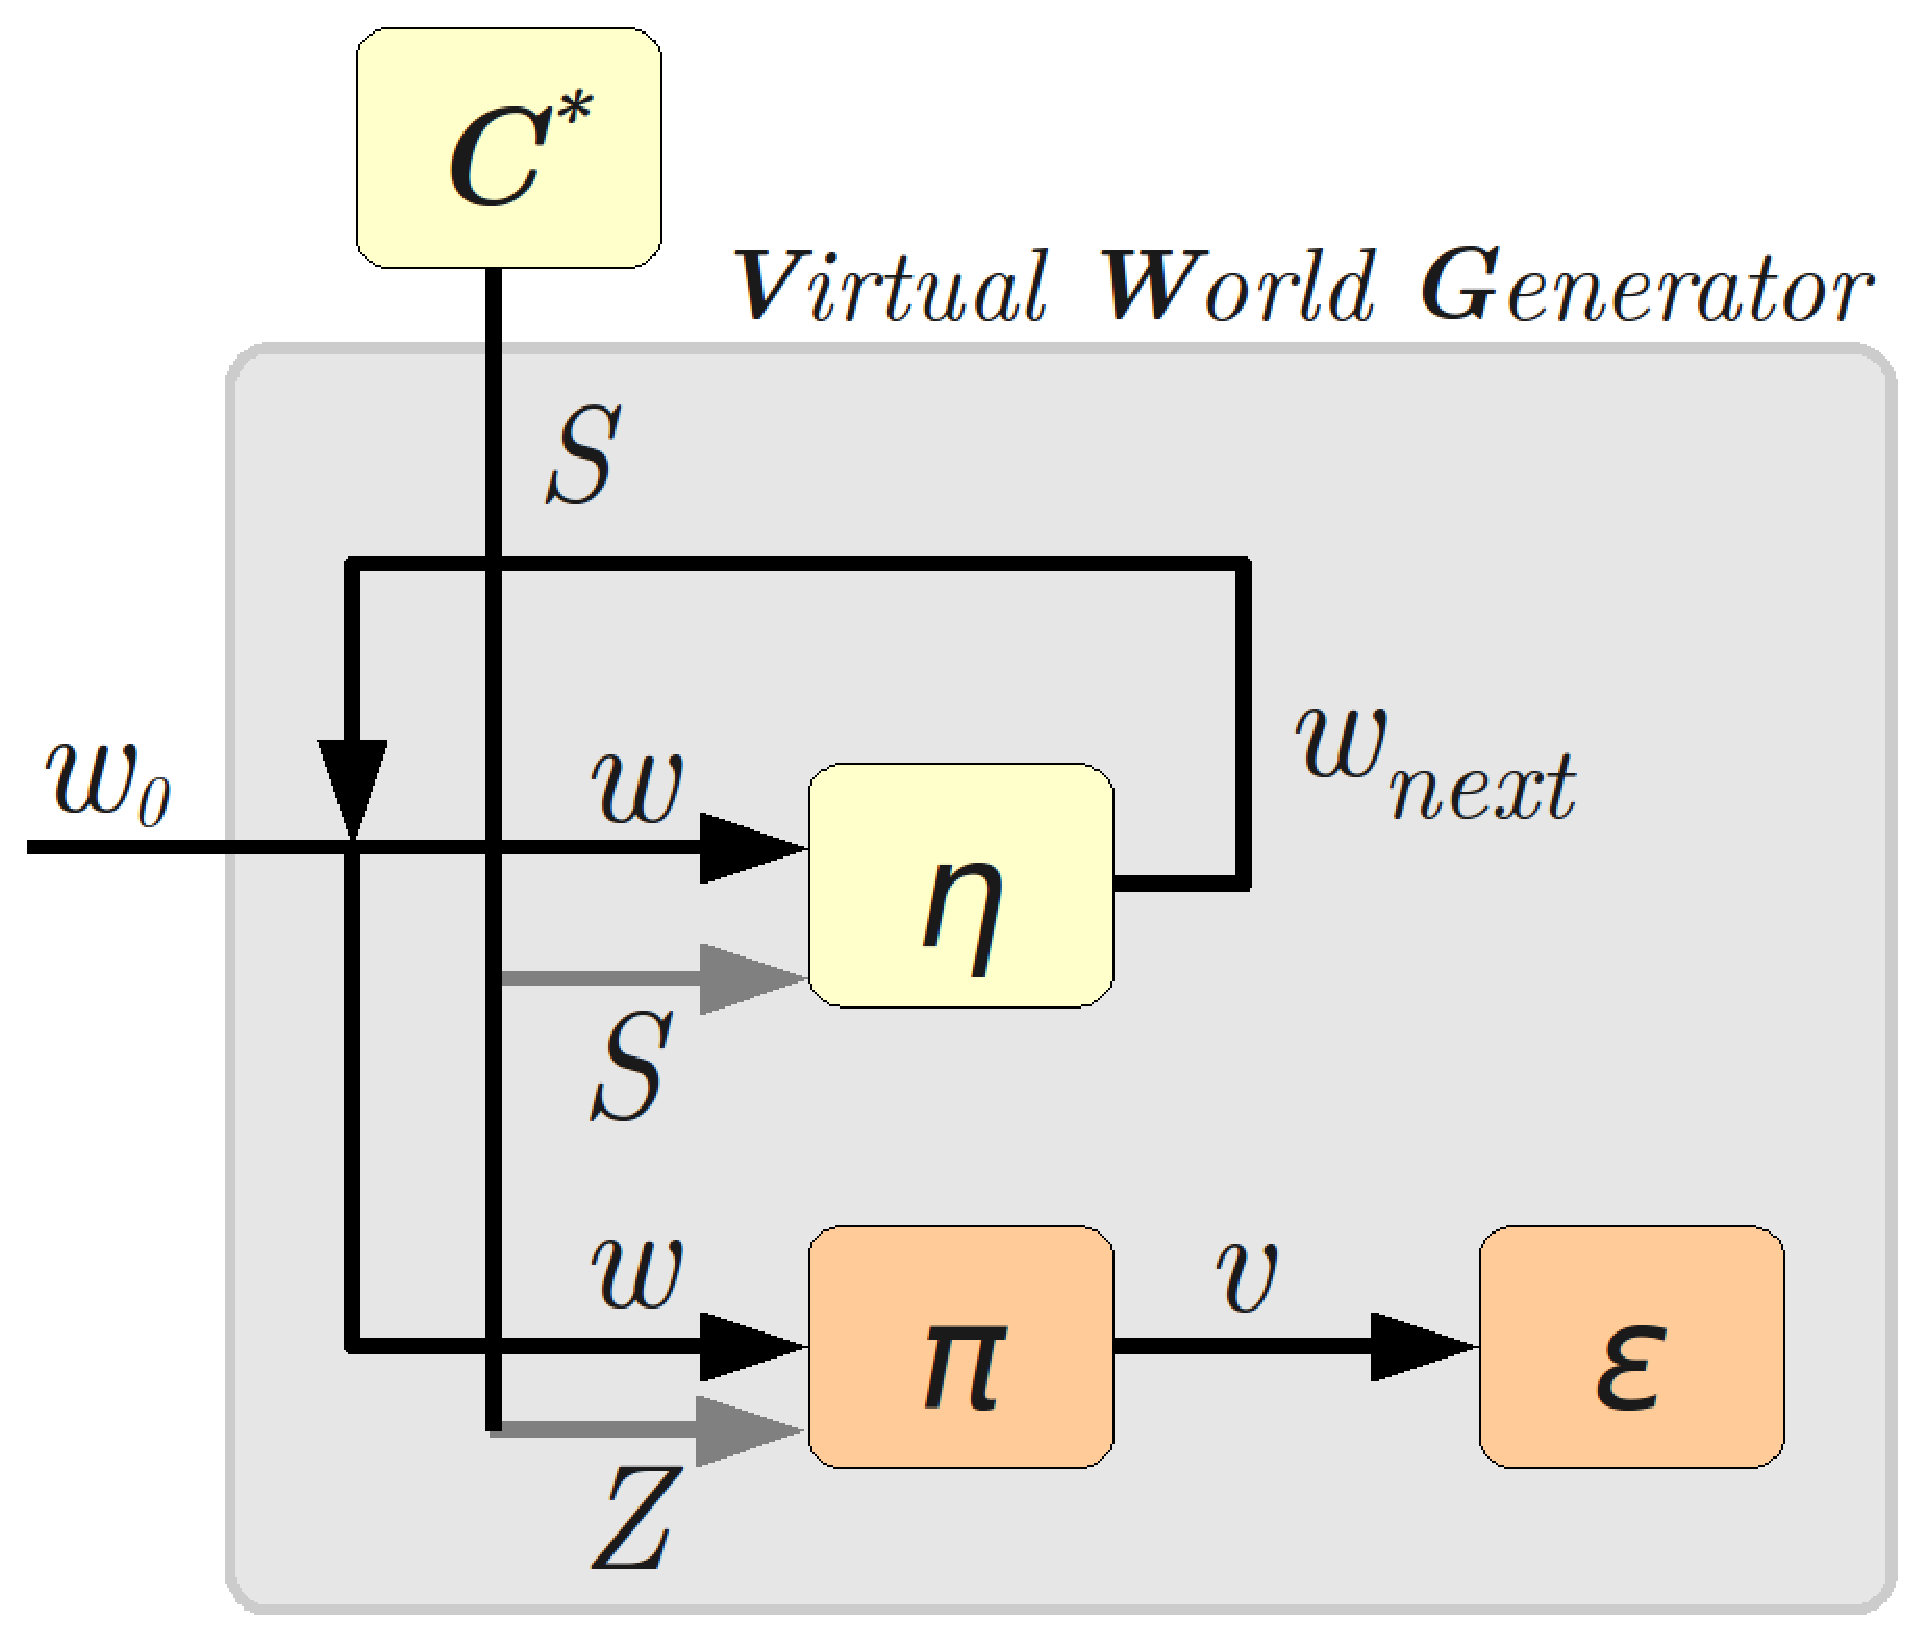
\includegraphics[width=0.8\linewidth]{figure3}
    \end{tabular}
    \caption{\label{fig:diagram} Virtual worlds generation algorithm}
\end{figure}


This formalization of the system has two main consequences. First, the scene definition is
separated from the hardware-dependent characteristics of components. The functions $\alpha$,
$\beta$ and $\delta$ provide the independence from the visualization system, and the event
generators provide the independence from the hardware input devices. Secondly, due to the fact that
there is an specific scheme to define the features of a system, the different system elements can be
reused easily in other areas of application.

%___________________________________________________________________________
\section{Case Study
\label{sec:case_study}}
%___________________________________________________________________________

This example is an application that simulates fires in forests with animals caused by lightning. It could be
used to analize the best distribution of trees to reduce the number of burnt trees \cite{John2007}.
It is important to notice that we are not actually interested in the problem of fire simulation,
but rather in defining a graphics system using the proposed model and all the concepts presented in
this paper. Therefore, it studies the ease of system modeling, expansion, portability and system
independence from hardware and other aspects of graphical representation.

%___________________________________________________________________________
\subsection{Problem Description
\label{sec:description_problem}}
%___________________________________________________________________________

Let $(i, j)$ be the cells of a 2D grid representing a squared world. At each cell, a tree can grow
with a given probability $g$. Bolts of lightning can also fall on a $(i, j)$ position
with a probability $f$. In this case, if there is a tree, it will burn as well as
the trees around it, in a chain reaction. 
Moreover, there are rabbits that can move through the forest. 
Theses rabbits will be dead if they occupie the same cell as a burning tree. 
An example can be seen in Figure \ref{fig:examplesDifferentSimulationState}.

\begin{figure}[htb]
    \centering
    \begin{tabular}{cc}
        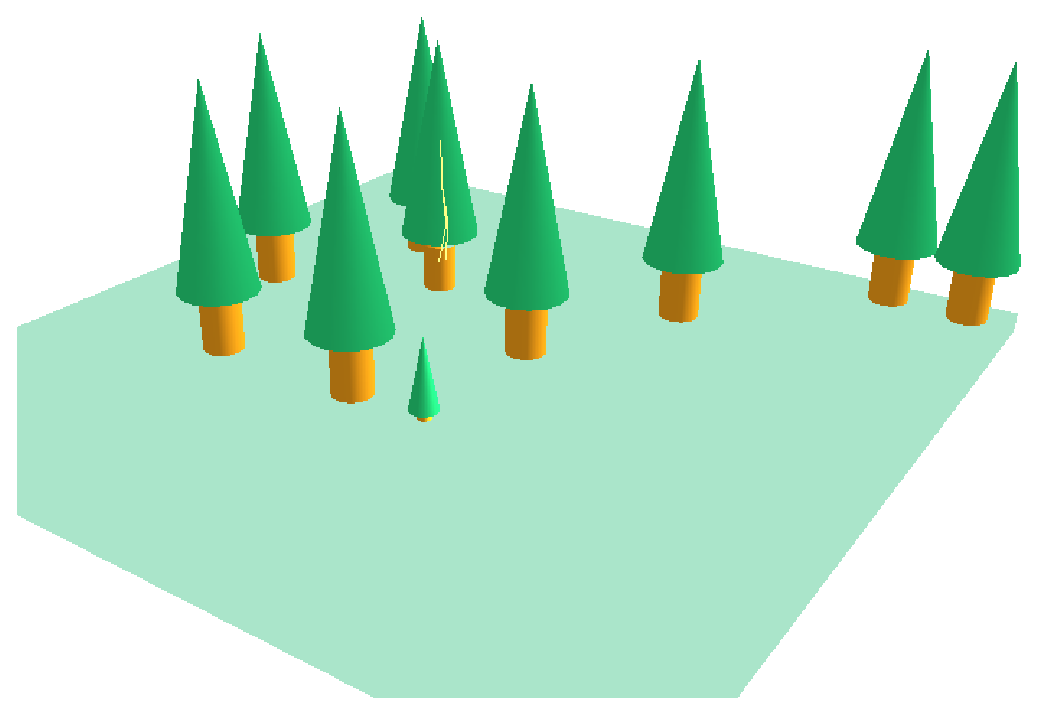
\includegraphics[width=3.5cm]{figure1} &
        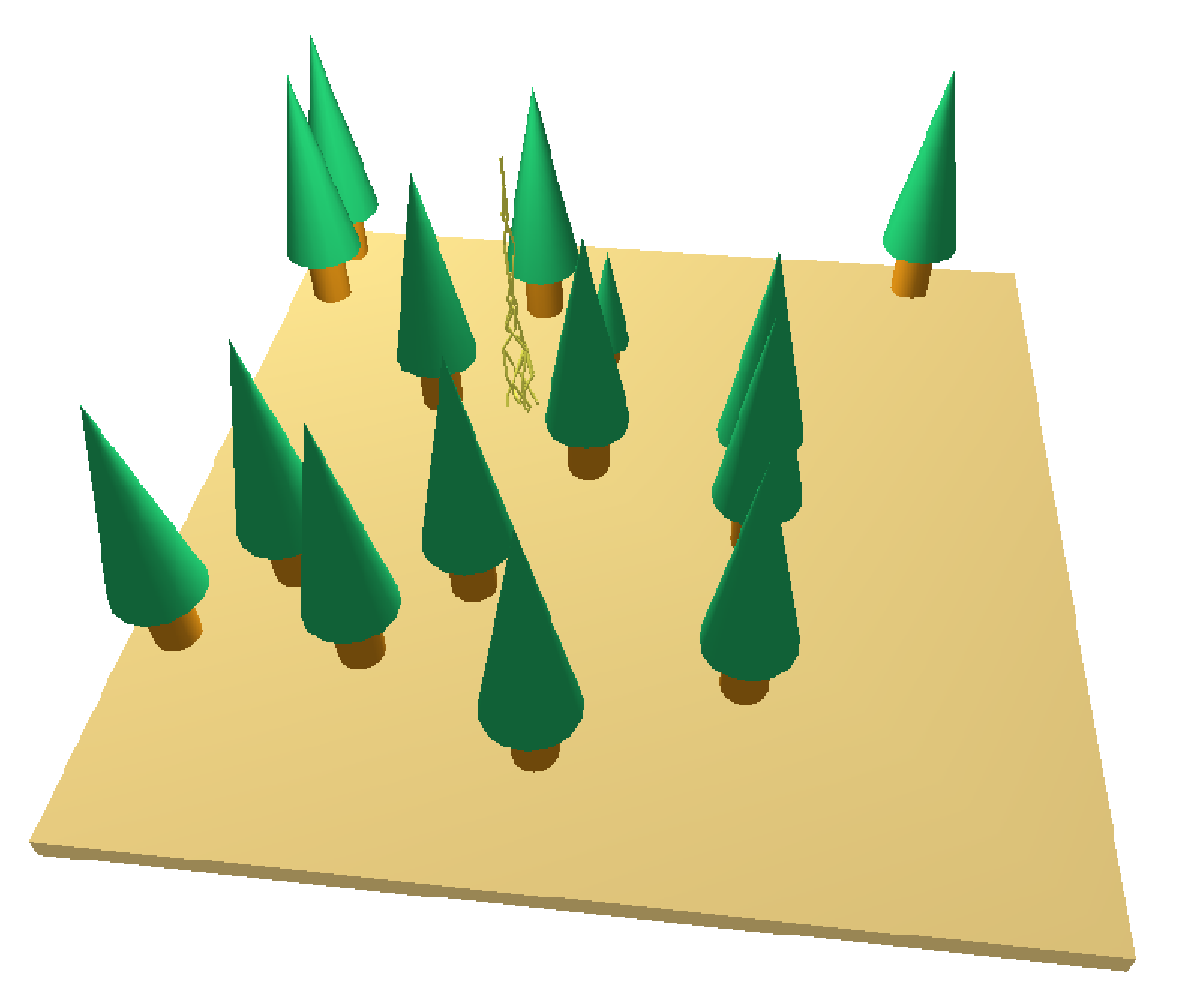
\includegraphics[width=3.5cm]{figure2}
    \end{tabular}
    \caption{\label{fig:examplesDifferentSimulationState} Examples of different simulation states}
\end{figure}

To model this example with our proposal, four main elements need to be defined. First, the graphic
primitives must be defined to show the visual elements on the rendering system. Second, it is
necessary to define events to run actor activities. These events include the necessary information
to develop their activity. After that, it is necessary to design the event generators that separate the
interactive system from the origin of the events (mouse, keyboard, physics engine and so on). 
Finally, it is necessary to define the actors included in the scene. 
These elements are used by the system to evolve over time.

%___________________________________________________________________________
\subsection{System Formalization
\label{sec:formalization_system_model}}
%___________________________________________________________________________

Following the steps described above, the different elements of the system are defined.

%___________________________________________________________________________
\subsubsection{Primitives and Transformations
\label{sec:primitivesandtransf}}

The graphical elements that can appear in the scene are: the grid (that is, the ground), the trees
(they can have three different graphical representation depending on their state), the bolts of
lightning and the rabbits. Therefore, six primitives are needed to represent these elements. They are shown in
Table \ref{tab:definitionPrimitives}.

\begin{table}[h]
\begin{center}
\begin{small}
\begin{tabular}{|l|l|}

    \hline \itshape Primitive & \itshape Description\\
    \hline $PrimTree$ & Draw a tree\\
    \hline $PrimBurningTree$ & Draw a burning tree\\
    \hline $PrimGrowningTree$ & Draw a growing tree\\
    \hline $PrimBoltLightning$ & Draw a bolt of lightning\\
    \hline $PrimRabbit$ & Draw a rabbit\\
    \hline $PrimGridNN$ & Draw a grid of NxN \\
    \hline

\end{tabular}
\end{small}
\caption{Definition of primitives
\label{tab:definitionPrimitives}}
\end{center}
\end{table}

To manipulate the primitives two transformations are needed: 
translation (used to move trees, bolts and rabbits), 
and scaling (used to simulate the growth of a tree). 
The transformations are shown in Table \ref{tab:definitionTransformations}:

\begin{table}[h]
\begin{center}
\begin{small}
\begin{tabular}{|l|l|}

    \hline \itshape Transformations & \itshape Description\\
    \hline $Translate_{(i,j)}$ & Translate to $(i,j)$ position of grid\\
    \hline $Scale_{s}$ & Scale a $s$ factor\\
    \hline

\end{tabular}
\end{small}
\caption{Definition of transformations
\label{tab:definitionTransformations}}
\end{center}
\end{table}


The functions ${\alpha}$, ${\beta}$ and ${\delta}$ define the semantics for these primitives and transformations. 
They are implemented as functions containing calls to a graphics library (in this case OpenGL). 
This way, the number of primitives and transformations can be easily extended just implementing the corresponding functions
${\alpha}$, ${\beta}$ and ${\delta}$.

%___________________________________________________________________________
\subsubsection{Events
\label{sec:events}}

Events are used to produce the necessary activity of the system. They are described by an
identifier and a set of data. Their aim is to produce certain activities of the actors that compose
the scene. The events defined for this example are shown in Table \ref{tab:eventDefinition}.


\begin{table}[h]
\begin{center}
\begin{small}
\begin{tabular}{|p{0.1\linewidth}|p{0.35\linewidth}|p{0.35\linewidth}|}

    \hline
    \itshape Type &
    \itshape Meaning &
    \itshape Associated data\\

    \hline
    $frame$ &
    Event generated every frame
    &
    Increasing time since previous frame event\\

    \hline
    $tree$ &
    Create a tree at a given position &
    Grid position $(i,j)$ where the tree is created \\

    \hline
    $bolt$ &
    Create a bolt of lightning at a given position &
    Grid position $(i,j)$ where the bolt of lightning is created\\

    \hline
    $rabbit$ &
    Create a rabbit at a given position &
    Rabbit identifier and the grid position $(i,j)$ where the rabbit is created\\

    \hline
    $kill$ &
    Kill a rabbit with a specific identifier &
    Identifier of the rabbit to kill\\
    \hline
    $draw$ &
    Draw using the graphics system &
    Void\\

    \hline

\end{tabular}
\end{small}
\caption{Events definition
\label{tab:eventDefinition}}
\end{center}
\end{table}

%___________________________________________________________________________
\subsubsection{Event Generators
\label{sec:generators}}

The next step is to define the event generators. 
They create the events described in the previous section. 
All generators share a table that has information about the elements in the forest. 
This table, called \textit{Positions Table (PT)}, has three fields: 
the element unique identifier (id), 
the element position (pos) and 
the element type (tree, burning tree, bolt of lightning or rabbit).

\begin{enumerate}

\item Frame event generator:
This generator has the responsibility of animating the system. Every time
instant, it generates an event $e^{frame}$ that is usually associated with some type of transformation of primitives.
Thus, it changes the appearance of an actor over time. In this example, the transformation will be the scaling of an element.

\[C_{frame} = \{ e^{frame} \ \mathit{each \ frame} \} \]

\item Collision event generator:
They analyze if a rabbit is in the same cell as a burning tree 
or if a bolt of lightning strike up a tree. 
In this case, the generator sends a kill event to the rabbit 
or an event to the tree to burn. 
The collision event generator uses the \textit{isBurning} function to calculate whether a rabbit should die.
This function is true if there is a burning tree in the same position as a rabbit. 
The collision event generator also calculates if a tree should be burned. 
In this case, it uses the \textit{IsBolt} function. 
Theses function uses the information stored in the \textit{PT} table, 
and returns true if there is a bolt of lightning at the same position as a tree. 


\[C_{collision}=
    \left\{
        \begin{array}{ll}
           e^{kill} & \forall x \in PT \\
            & \land \ x.type=rabbit \\
            & \land \ IsBurning(x.pos) = true \\
          e^{burn} & \forall x \in PT \\
            & \land \ x.type=tree \\
            & \land \ IsBolt(x.pos) = true
        \end{array}
    \right\}\\ \]

$e^{kill}$ has the rabbit identifier that must be killed and $e^{burn}$ has the tree identifier that must be burned.

\item Forest event generator:
This generator produces events to create trees, bolts of lightning and rabbits. Taking into account the
previous specification, trees are created with a probability $g$, lightning with a probability
$f$ and rabbits with a probability $r$. This generator is defined as:

\[C_{forest}=
    \left\{
        \begin{array}{ll}
            e^{tree} & with \ probability \ g \\
            e^{bolt} & with \ probability \ f \\
            e^{rabbit} & with \ probability \ r 
        \end{array}\right\}\\ \]

All the events created by this generator have an associated unique element identifier. 
They also add a new entry to the \textit{PT} table.

\item Visualization event generator:
This generator is necessary to visualize all the elements in the scene. This means that every
time a drawing order is received, the generator captures this order and produces an
event. At the same time, it sends the elements of the scene to draw in the graphics system.
It is defined as:

\[C_{visualization} = \{ e^{draw} \ \mathit{each \ drawing \ cycle} \} \]
\end{enumerate}

%___________________________________________________________________________
\subsubsection{Actors
\label{sec:actors}}

The last step is to specify the actors which compose the dynamic part of the system. 
As explained in section \ref{sec:rule4}, an actor is defined by its evolution function $\lambda$. 
If it has a graphical representation, it also needs a function $\theta$ to generate the primitives and the
transformations.

There are four actors in the scene: the forest, which represents the ground and manages all the other actors, the trees, the bolts of lightning and the rabbits.

The actor $Forest^{tree, bolt, rabbit, draw}$ can respond to four events. 
Three of them (create a tree, create a bolt of lightning and create a rabbit) 
are involved in its evolution function and the other one (draw the forest) 
in the visualization function. So, the evolution function for 
$Forest^{tree, bolt, rabbit, draw}$ includes the creation of a tree when 
it receives the event $e^{tree}$, 
the creation of a bolt of lightning when it receives the event $e^{bolt}$ 
and the creation of a rabbit when it receives the event $e^{rabbit}$. 
These events also contain the identifiers of the trees, 
the bolts of lightning or the rabbits to be created. 
This evolution function is defined in Table \ref{tab:tableForest}. 
The $e^{draw}$ event has been eliminated in the table for simplicity 
and $Forest^{tree,bolt,rabbit}$ is represented as $Forest^{t,b,r}$. 
The drawing function $\theta$ will be defined later.


\begin{table}[h!]
\begin{small}
\renewcommand{\arraystretch}{1.5}
\begin{tabular}{ | l | l |}
    \hline
    \itshape Actor & $Forest^{t,b,r}$ \\
    \hline
    \itshape Description & Represents the forest \\
    \hline
    \multicolumn{2}{|c|}
    {
      \renewcommand{\arraystretch}{1}
      $\begin{array}{l}
      \vspace{0.2cm}
      \lambda(Forest^{t,b,r}, e^{h}) =\\
      \left\{
        \begin{array}{ll}
            \vspace{0.2cm}
            Tree_{\langle gr, e^{tree}.id, 1 \rangle}^{frame,burn} \cdot Forest^{t,b,r}
                & \mathit{if} \ h = tree \\

            \vspace{0.2cm}
            Lightning_{\langle e^{bolt}.id, 1 \rangle}^{frame} \cdot Forest^{t,b,r}
                & \mathit{if} \ h = bolt \\
                
            \vspace{0.2cm}
            Rabbit_{\langle \cdot, e^{rabbit}.id\rangle}^{frame,kill} \cdot Forest^{t,b,r}
                & \mathit{if} \ h = rabbit \\

            Forest^{t,b,r}
                & \mathit{if} \ h \notin \lbrace tree,bolt,rabbit \rbrace \\
        \end{array}\right\}\end{array}$

    }\\
    \hline
\end{tabular}
\end{small}
\caption{Evolution function of the actor $Forest$
\label{tab:tableForest}}
\end{table}

The actor $Tree_{\langle st,id,nframe \rangle}^{frame,bolt,draw}$ (see Table \ref{tab:tableTree}) 
can also respond to three events 
(the frame event, the creation of a bolt of lightning and the draw event) and has three attributes. 
The first attribute, the state (\textit{st}), defines whether the tree is $growing$, $burning$ or $adult$. 
The second attribute corresponds to the $(i,j)$ position of the tree within the grid. 
The last attribute is used to store the current tree animation frame. 
The tree evolves depending on the received event and on its current attributes. 

For instance, when a tree is growing and receives a \textit{frame} event, 
the growing animation advances, unless the final animation frame ($N_{frames}$) is reached. 
On the contrary, when the tree state is $burning$, the animation is reversed by decreasing 
the $nframe$ attribute until 0 is reached 
(some other details about this animations will be discussed later). 
Finally, if a bolt of lightning is created at the
same position as a tree, the collision event generator sends a \textit{burn} event 
to change the tree state to $burning$.

\begin{table}[h!]
\begin{small}
\renewcommand{\arraystretch}{1.5}
\begin{tabular}{ | l | l |}
    \hline

    \itshape Actor & $Tree_{\langle st,pos,nframe \rangle}^{frame,burn}$ \\
    \hline

    \itshape Description & Represents a tree \\
    \hline

    \multicolumn{2}{|c|}
    {
    \renewcommand{\arraystretch}{1}
    $\begin{array}{l}
        \vspace{0.2cm}
        \lambda(Tree_{\langle st,pos,nframe \rangle}^{frame,burn},e^{h}) =\\
        \left\{
        \begin{array}{ll}
            Tree_{\langle growing,id,nframe+1 \rangle}^{frame,burn}
                  & \mathit{if} \ h=frame \\
                  & \ \wedge st = growing \\
                  \vspace{0.3cm}
                  & \ \wedge nframe < N_{frames} \\

            Tree_{\langle adult,id,N_{frames} \rangle}^{frame,burn}
                  & \mathit{if} \ h=frame \\
                  & \ \wedge st = growing \\
                  \vspace{0.3cm}
                  & \ \wedge nframe \geqslant N_{frames} \\

            Tree_{\langle burning,id,nframe-1\rangle}^{frame,burn}
                  & \mathit{if} \ h=frame \\
                  & \ \wedge st = burning \\
                  \vspace{0.3cm}
                  & \ \wedge nframe > 0 \\

            \epsilon & \mathit{if} \ h=frame \\
                 & \ \wedge st = burning \\
                 \vspace{0.3cm}
                 & \ \wedge nframe = 0 \\

            Tree_{\langle burning,id,nframe\rangle}^{frame,burn}
                 & \mathit{if} \ h=burn \\
                 \vspace{0.2cm}
                 & \ \wedge e^{burn}.id = id \\

            Tree_{\langle st,pos,nframe \rangle}^{frame,burn}
                & \mathit{if} \ h \notin {frame,burn}\\
    \end{array}\right\}\end{array}$
}\\
    \hline
\end{tabular}
\end{small}
\caption{Evolution function of the actor $Tree$
\label{tab:tableTree}}
\end{table}

Table \ref{tab:tableBoltOfLightning} defines the evolution function of a bolt of lightning. 
In this case, it can respond to the $frame$ and the $draw$ events. 
It has two attributes: the bolt of lightning identifier and the animation frame. 
The lightning animation is defined similarly to that of the trees.


\begin{table}[h!]
\begin{small}
\renewcommand{\arraystretch}{1.5}
\begin{tabular}{ | l | l |}

    \hline
    \itshape Actor & $Lightning_{\langle id,nframe \rangle}^{frame}$ \\
    \hline
    \itshape Description & Represents the bolt of lightning \\
    \hline
    \multicolumn{2}{|c|}
    {
    \renewcommand{\arraystretch}{1}
    $\begin{array}{l}
    \vspace{0.2cm}
    \lambda(Lightning_{\langle id,nframe \rangle}^{frame},e^{h}) = \\
    \left\{
    \begin{array}{ll}
        Lightning_{\langle id,nframe+1 \rangle}^{frame}
                & \mathit{if} \ h=frame \\
                \vspace{0.3cm}
                &  \wedge \ nframe < N_{frames} \\

        \epsilon & \mathit{if} \ h=frame \\
                 \vspace{0.3cm}
                 & \wedge  \ nframe \geqslant N_{frames} \\

        Lightning_{\langle id,nframe \rangle}^{frame}
                 & \mathit{if} \ h \neq frame\\

    \end{array}\right\}\end{array}$

    }\\
    \hline
\end{tabular}
\end{small}
\caption{Evolution function of the actor $Lightning$
\label{tab:tableBoltOfLightning}}
\end{table}

The last actor to consider is the rabbit. 
Its evolution function is defined in Table \ref{tab:tableRabbit}. 
This actor decides the direction to take whenever he receives a \textit{frame} event.
This behaviour is controlled by a function called $DecideDesire(e^{frame})$, 
which form part of the artificial intelligence engine. 
In this case, this function implements a random behaviour which could be left, right, front, back or stop. 
This function could be replaced by a more advanced behavior. 
For example, run in the opposite direction when the actor is next to a burning tree.


\begin{table}[h!]
\begin{small}
\renewcommand{\arraystretch}{1.5}
\begin{tabular}{ | l | l |}

    \hline
    \itshape Actor & $Rabbit_{\langle desire, id \rangle}^{frame,kill}$ \\
    \hline
    \itshape Description & Represents a rabbit \\
    \hline
    \multicolumn{2}{|c|}
    {
    \renewcommand{\arraystretch}{1}
    $\begin{array}{l}
    \vspace{0.2cm}
    \lambda(Rabbit_{\langle desire, id \rangle}^{frame},e^{h}) = \\
    \left\{
    \begin{array}{ll}
        Rabbit_{\langle DecideDesire(e^{frame}),id \rangle}^{frame,kill}
                & \mathit{if} \ h=frame \\
        \epsilon & \mathit{if} \ h=kill \\
    \end{array}\right\}\end{array}$

    }\\
    \hline
\end{tabular}
\end{small}
\caption{Evolution function of the actor $Rabbit$
\label{tab:tableRabbit}}
\end{table}

Finally, Table \ref{tab:defintionDrawFunctions} shows the definition of the drawing functions $\theta$. 
These functions are used to obtain the set of primitives and transformations representing the visual aspect of the actors. 
They are helped by \textit{PosPT(id)} (which returns the position of an element) 
and \textit{PosWithDesirePT(desire,id)} (which returns the position of an element and updates its position using the last decision).
For example, if the decision is going up, the element will increment its \textit{Y} position;
if the decision is going down, it will decrement the \textit{Y} position; and so on. 

\begin{table}[h!]
\begin{center}
\begin{small}
\renewcommand{\arraystretch}{1.5}
\begin{tabular}{|l|}

    \hline

    $\theta (Forest^{draw}, e^{h})=
        \left\{
          \begin{array}{ll}
            \mathit{PrimGridNN} & \mathit{if} \ h = draw\\
            \epsilon            & \mathit{if} \ h \neq draw\\
          \end{array}
        \right\}$ \\

    \hline

      \renewcommand{\arraystretch}{1}
      $\begin{array}{ll}
      \vspace{0.2cm}
      \theta (Tree_{\langle st,id,nframe \rangle}^{draw}, e^{h})= \\
      \left\{
      \begin{array}{ll}
        Translate_{PosPT(id)}(S_{s}(\mathit{PGTree}))
                        &  \wedge  \  h = draw\\  \vspace{0.2cm}
                        & \ \mathit{if} \  st = growing\\

        Translate_{PosPT(id)}(S_{s}(\mathit{PBTree}))
                           &  \wedge \  h = draw\\ \vspace{0.2cm}
                           & \ \mathit{if} \ st = burning \\

        Translate_{PosPT(id)}(\mathit{PrimTree})
                        &   \wedge  \ h = draw\\ \vspace{0.2cm}
                        & \ \mathit{if} \ st = adult \\

        \epsilon        & \mathit{if} \ h \neq draw\\
      \end{array}
      \right\}\end{array}$  \\
    Where:\\
    \begin{scriptsize}\vspace{-0.1cm}$PGTree = PrimGrowingTree$ \end{scriptsize} \\
    \begin{scriptsize}$PBTree = PrimBurningTree$ \end{scriptsize} \\

    \hline

      $\theta (Ligthning_{\langle id,nframe \rangle}^{draw}, e^{h})=$\\
      $
      \left\{
      \begin{array}{ll}
        Translate_{PosPT(id)}(S_{s}(\mathit{PrimBoltLightning}))
                 & \mathit{if} \ h = draw \\
        \epsilon & \mathit{if} \ h \neq draw\\
      \end{array}
      \right\}$ \\

    \hline

      $\theta (Rabbit_{\langle desire, id \rangle}^{draw}, e^{h})=$\\
      $
      \left\{
      \begin{array}{ll}
        Translate_{PosWithDesirePT(desire,id)}(\mathit{PrimRabbit})
                 & \mathit{if} \ h = draw \\
        \epsilon & \mathit{if} \ h \neq draw\\
      \end{array}
      \right\}$ \\

    \hline
\end{tabular}
\end{small}
\caption{Definition of the drawing function $\pi$
\label{tab:defintionDrawFunctions}}
\end{center}
\end{table}

In Table \ref{tab:defintionDrawFunctions}, the actor $Forest$ is drawn as a $PrimGridNN$ primitive.
In the case of trees, the used primitives are $PrimGrowingTree$, $PrimBurningTree$ or $PrimTree$
depending on the tree state. 
In the case of $growing$ or $burning$ states, a scaling transformation is also introduced. 
The growing scale factor $s$ is defined by the
expression $s = \frac{nframe}{N_{frame}}$, so the higher the $nframe$ value, the higher the factor
$s$. From this expresion and from the function in Table \ref{tab:tableTree}, it can be deduced that
the $Tree$ size is increased when it receives the event $e^{frame}$ and it is growing, and when the
$Tree$ is in burning state, this effect is inverse. In the case of $Lightning$ the animation is
done in the same way. 
The rabbit is drawn using the \textit{PrimRabbit} primitive 
and his drawing process is similar to those already explained.
This example shows how the attributes of an actor are used to change its
behaviour.

In general, actors animations always depend on $frame$. 
It modifies the current state of the actor to change its representation and thus, 
it performs the animation.



%___________________________________________________________________________
\subsection{Example of the Evolution of the Algorithm
\label{sec:example_algorithm}}
%___________________________________________________________________________

Table \ref{tab:exampleAlgorithmEvolution} shows the first iterations in the evolution of the
algorithm for this example. The algorihtm starts with the initial string $w_0=Forest^{tree,
bolt,rabbit, draw}$. It is the first string to be processed in the algorithm. From this initial state, the
system evolves over time (See algorithm scheme in Section \ref{sec:system_algorithm}). Two events
are always generated at every step to make the system evolve and to draw it on the display:
$e^{frame}$ and $e^{draw}$. Besides, at some iterations, random events to create trees and bolts of
lightning are also generated.

\begin{table*}[ht]
\begin{center}
{\small
\hfill{}
    \renewcommand{\arraystretch}{1.5}
\begin{tabular}{|p{0.01\linewidth}|l|l|l|p{0.3\linewidth}|}

\hline
\textit{It.} & \textit{Evolution Strings} & \textit{Draw Strings} & \textit{Generated Events} & \textit{Observations}\\

    \hline
    1 &
    $Forest^{tree, bolt, rabbit, draw}$ &
    &
    $e^{draw}, e^{frame}, e^{tree}$ &
    Initial String. Apart from $e^{draw}$ and $e^{frame}$, $e^{tree} = (tree0)$ is received (random event, create a tree with tree0 identifier at (1,2) position).\\

    \hline
    2 &
    $\begin{array}{l}
            Tree_{\langle gr, tree0, 1 \rangle}^{frame,bolt,draw}\\
             \cdot Forest^{tree, bolt, rabbit, draw}
      \end{array}$
      &
    $PrimGridNN$ &
    $e^{draw}, e^{rabbit}, e^{frame}$ &
    A tree is generated in the evolution string. The primitive $PrimGridNN$ is added to the draw string. $e^{rabbit}$ is create with rabbit0 identifier at position (2,1)\\

    \hline
    3 &
    $\begin{array}{l}
            Tree_{\langle gr, tree0, 2 \rangle}^{frame,bolt,draw}\\
             \cdot Rabbit_{\langle \cdot,rabbit0 \rangle}^{frame,kill,draw} \\
             \cdot Forest^{tree, bolt, rabbit, draw} 
      \end{array}$
      &
    $\begin{array}{l}
            Translate_{(1,2)}(S_{1}(PGTree))\\
            \cdot PrimGridNN
      \end{array}$
      &
    $e^{draw}, e^{frame}$ &
    The tree animation evolves. The tree is drawn, adding, scaling and translating a $PrimGrowingTree$ primitive. A rabbit is showed with rabbit0 identifier and desire stop.\\

    \hline
    4 &
    $ \begin{array}{l}
            Tree_{\langle gr, tree0, 3 \rangle}^{frame,bolt,draw}\\
             \cdot Rabbit_{\langle left,rabbit0 \rangle}^{frame,kill,draw}\\
             \cdot Forest^{tree, bolt, rabbit, draw}
      \end{array}$
    &
    $\begin{array}{l}
            Translate_{(1,2)}(S_{2}(PGTree))\\
            \cdot Translate_{(2,1)}(PrimRabbit)\\
            \cdot PrimGridNN
      \end{array}$
    &
    $e^{draw}, e^{frame}, e^{bolt}$ &
    The tree animation goes on evolving. $e^{bolt} = (bolt0)$ is received (random event, create a bolt of lightning at (2,2) position). The rabbit desires to go to left direction\\

    \hline
    5 &
    $\begin{array}{l}
            Tree_{\langle adult, tree0, 3 \rangle}^{frame,bolt,draw}\\
            \cdot Rabbit_{\langle \cdot,rabbit0 \rangle}^{frame,kill,draw}\\
            \cdot Lightning_{\langle bolt0, 1 \rangle}^{frame,draw}\\
            \cdot Forest^{tree, bolt, rabbit, draw}
      \end{array}$
    &
    $\begin{array}{l}
            Translate_{(1,2)}(S_{3}(PGTree))\\
            \cdot Translate_{(1,1)}(PrimRabbit)\\
             \cdot PrimGridNN
      \end{array}$
    &
    $e^{draw}, e^{frame}$ &
    A bolt of lightning is generated. After 3 frames, the tree changes its state to adult. Rabbit changes his position to (1,1) and his next desire is stop.\\

    \hline
    6 &
    $\begin{array}{l}
             Tree_{\langle adult,tree0,3 \rangle}^{frame,bolt,draw}\\
             \cdot Rabbit_{\langle up,rabbit0 \rangle }^{frame,kill,draw}\\
			 \cdot Lightning_{\langle bolt0, 2 \rangle}^{frame,draw}\\
             \cdot Forest^{tree, bolt, rabbit, draw}
      \end{array}$
    &
    $\begin{array}{l}
            Translate_{(1,2)}(PrimTree)\\
            \cdot Translate_{(1,1)}(PrimRabbit)\\
            \cdot Translate_{(2,2)}(S_{1}(\mathit{PBLight}))\\
            \cdot PrimGridNN
      \end{array}$
    &
    $e^{draw}, e^{frame}$ &
    The lightning animation evolves. The lightning is drawn, adding, scaling and translating a $PrimBoltLightning$ primitive. The tree primitive is changed to draw an adult tree $PrimTree$. The rabbit desires to go to up.\\

    \hline
    7 &
    $\begin{array}{l}
             Tree_{\langle adult,tree0,3 \rangle}^{frame,bolt,draw}\\
             \cdot Rabbit_{\langle eup,rabbit0 \rangle}^{frame,kill,draw}\\
	         \cdot Lightning_{\langle bolt0, 3 \rangle}^{frame,draw}\\
             \cdot Forest^{tree, bolt, rabbit, draw}
      \end{array}$
    &
    $\begin{array}{l}
            Translate_{(1,2)}(PrimTree)\\
		    \cdot Translate_{(1,2)}(PrimRabbit)\\
            \cdot Translate_{(2,2)}(S_{2}(\mathit{PBLight}))\\
            \cdot PrimGridNN
      \end{array}$
    &
    $e^{draw}, e^{frame}$ &
    The lightning animation goes on evolving. The rabbit go up another one.\\

    \hline
    8 &
    $\begin{array}{l}
             Tree_{\langle adult,tree0,3 \rangle}^{frame,bolt,draw}\\
             \cdot Rabbit_{\langle \cdot,rabbit0 \rangle}^{frame,kill,draw}\\
             \cdot Forest^{tree, bolt, rabbit, draw}
      \end{array}$
    &
    $\begin{array}{l}
            Translate_{(1,2)}(PrimTree)\\
		    \cdot Translate_{(1,3)}(PrimRabbit)\\
            \cdot Translate_{(2,2)}(S_{3}(\mathit{PBLight}))\\
            \cdot PrimGridNN
      \end{array}$
    &
    $e^{draw}, e^{frame}$ &
    The lightning finishes its evolution and it is eliminated from the evolution string.\\

    \hline
    9 &
    $\begin{array}{l}
             \cdot Tree_{\langle adult,tree0,3 \rangle}^{frame,bolt,draw}\\
             \cdot Rabbit_{\langle down,rabbit0 \rangle}^{frame,kill,draw}\\
             \cdot Forest^{tree, bolt, rabbit, draw}
      \end{array}$
    &
    $\begin{array}{l}
            Translate_{(1,2)}(PrimTree)\\
		    \cdot Translate_{(1,3)}(PrimRabbit)\\
            \cdot Translate_{(2,2)}(S_{3}(\mathit{PBLight}))\\
            \cdot PrimGridNN
      \end{array}$
    &
    $e^{draw}, e^{frame}$ &
    Finally, the bolt of lightning is also eliminated from the draw string.\\

    \hline
    ... &
    \multicolumn{4}{|l|}
    {
      And so on...
    }\\
    \hline
\end{tabular}}
\hfill{}
\caption{Example of the first steps in the evolution of the algorithm
\label{tab:exampleAlgorithmEvolution}}
\end{center}
\end{table*}

\begin{figure}[htb]
    \begin{tabular}{cc}
        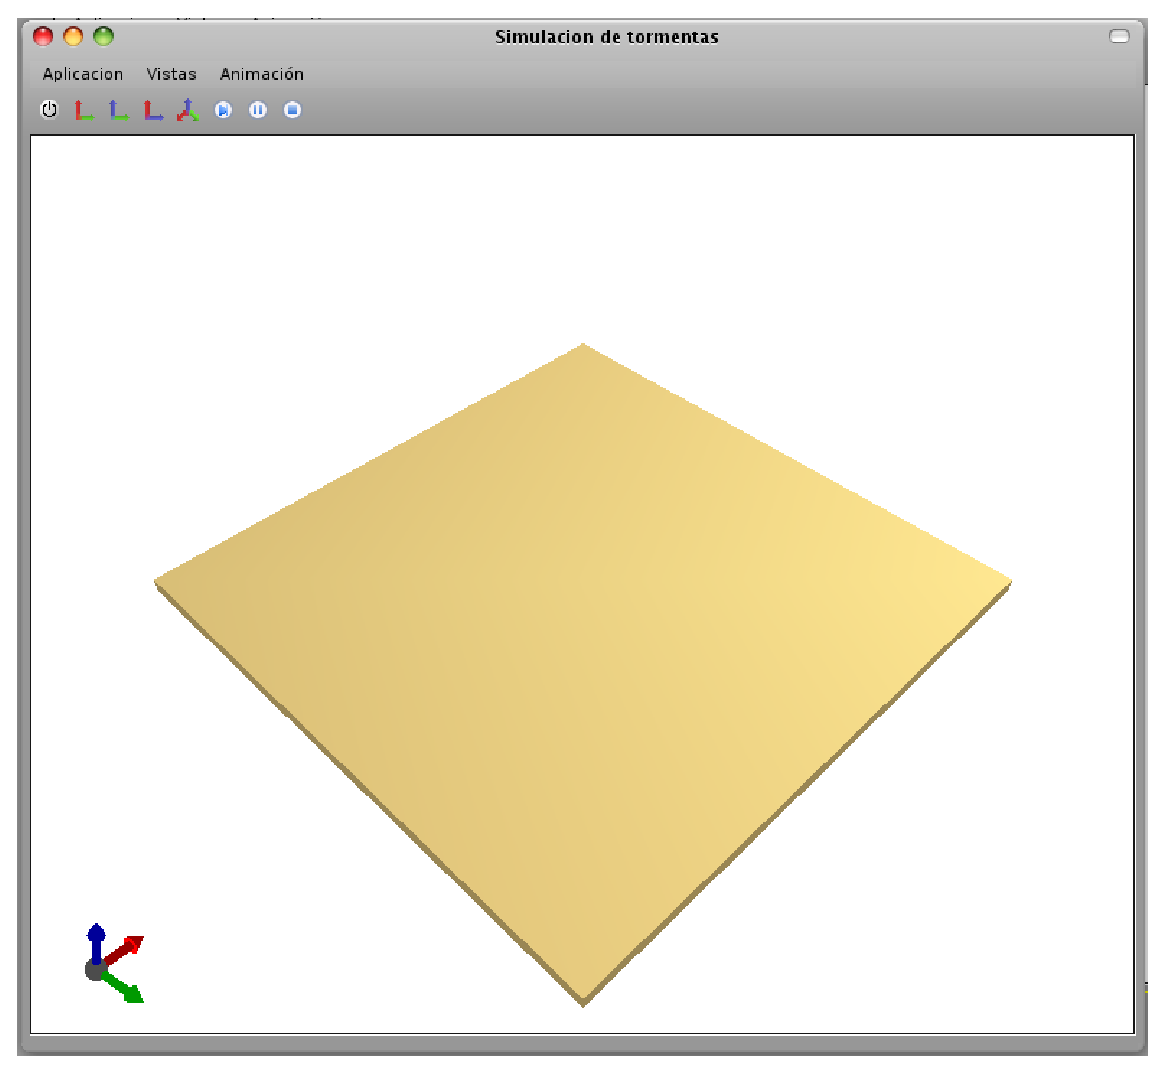
\includegraphics[width=0.45\linewidth]{figure4} &
        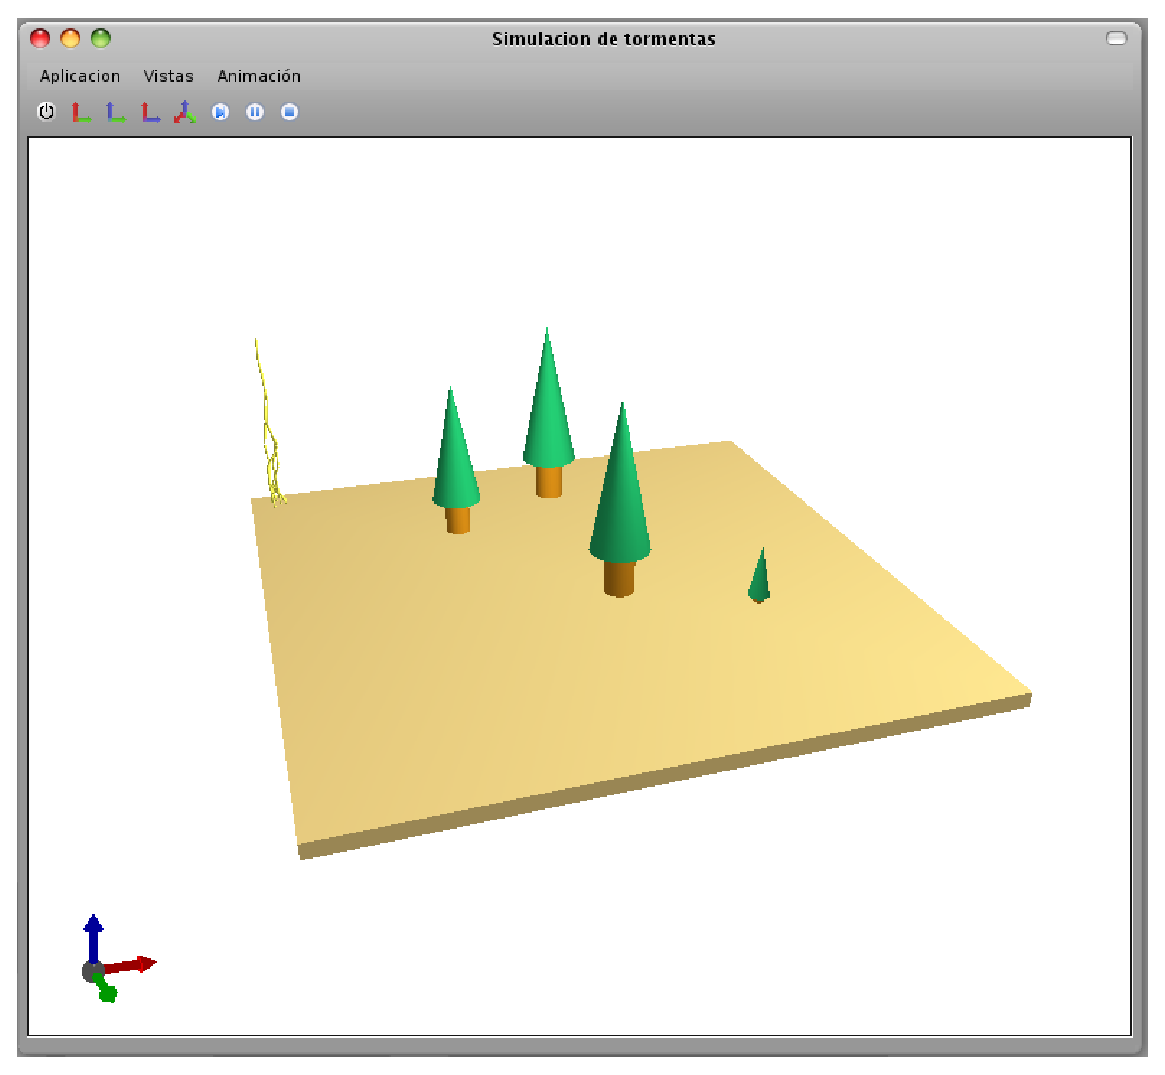
\includegraphics[width=0.45\linewidth]{figure5} \\
        \small{(a)} & \small{(b)} \\
        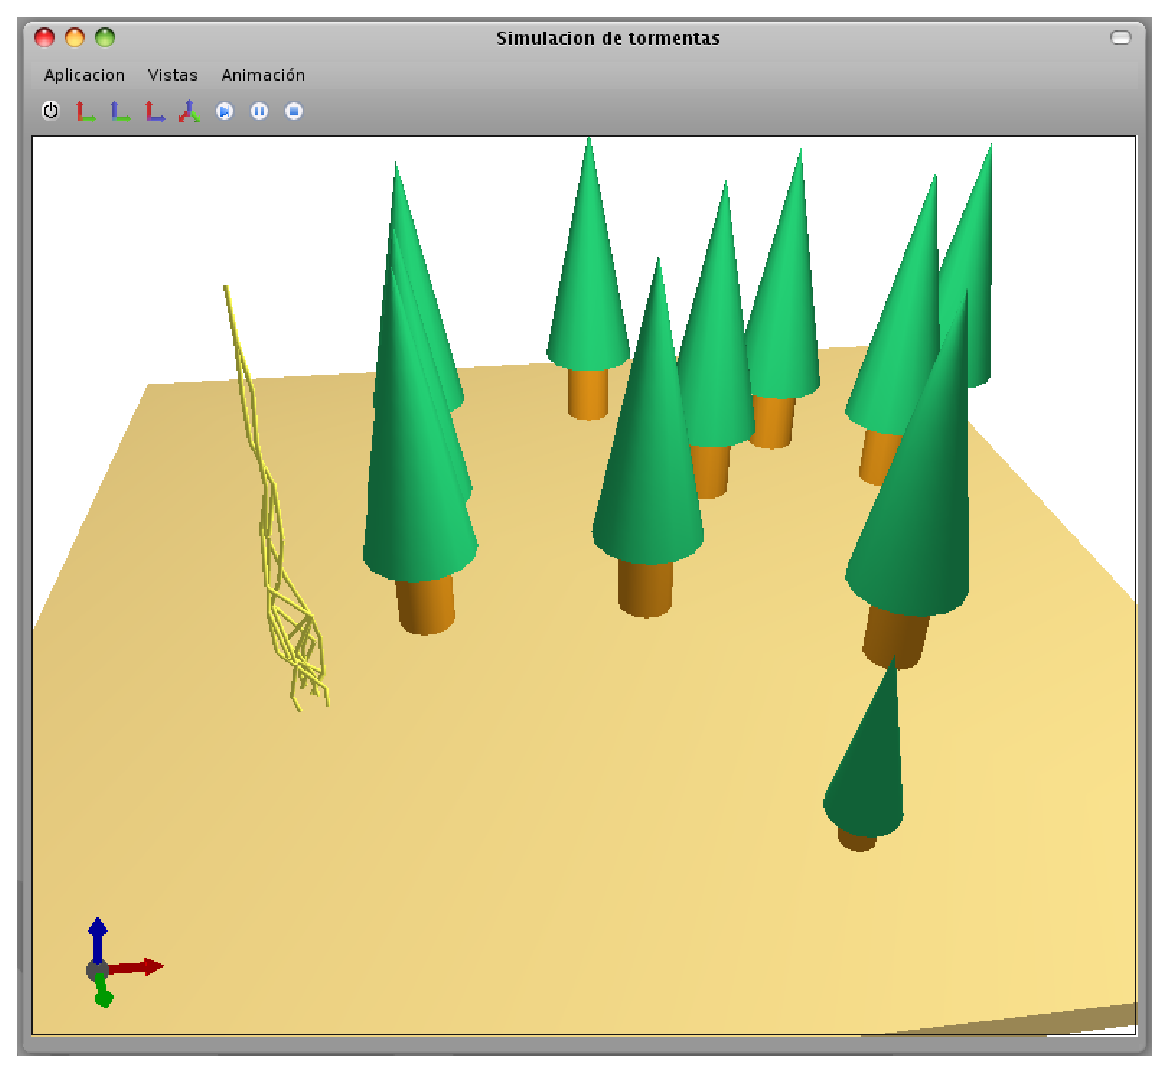
\includegraphics[width=0.45\linewidth]{figure6} &
        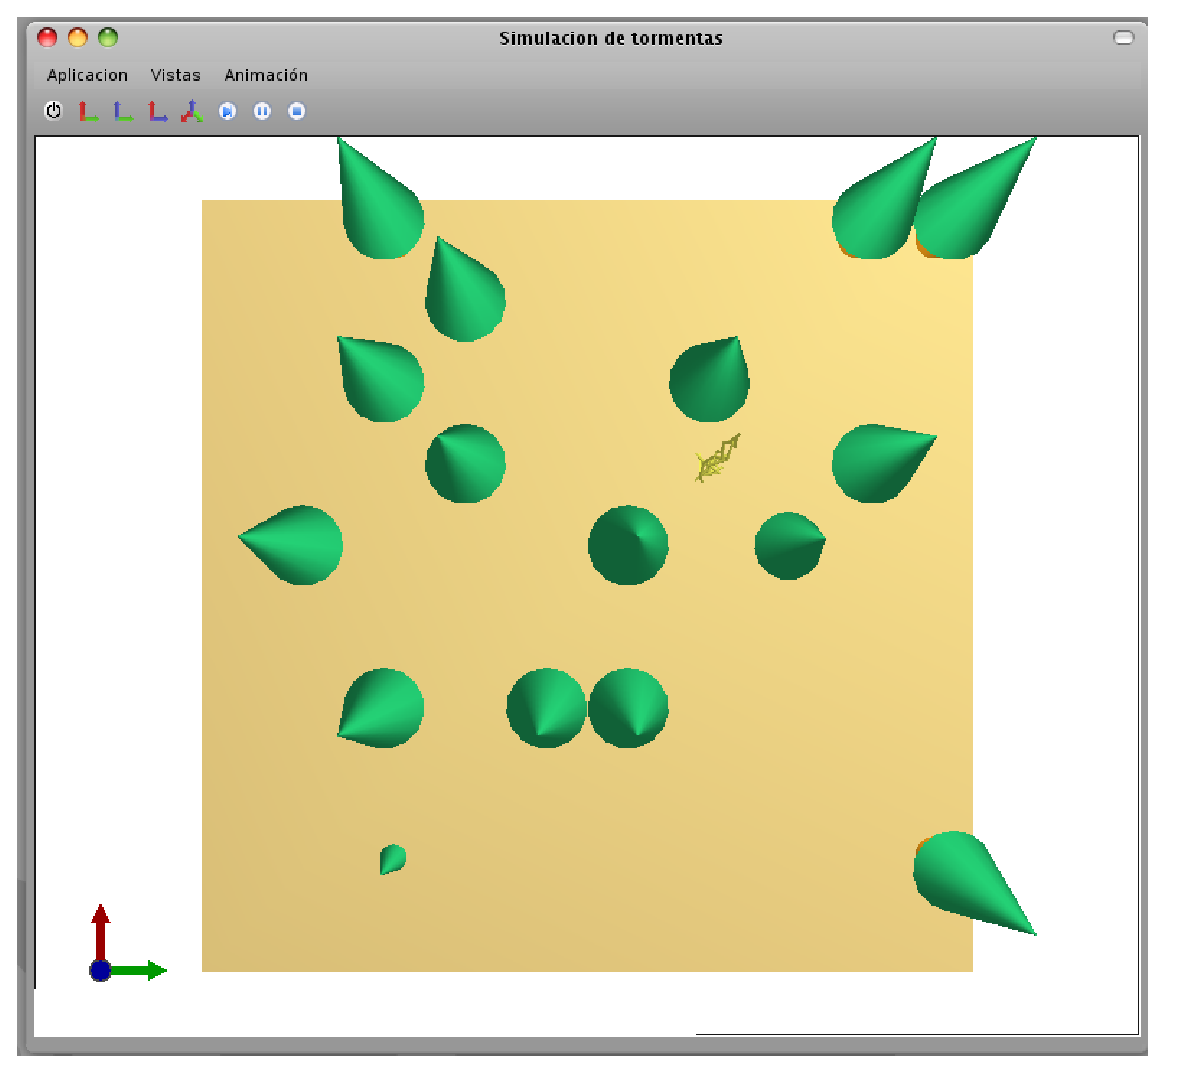
\includegraphics[width=0.45\linewidth]{figure7} \\
        \small{(c)} & \small{(d)} \\
    \end{tabular}
    \caption{\label{fig:programView}
    Some application views where it can be seen the evolution of forrest}
\end{figure}


%___________________________________________________________________________
\section{Conclusions and Future Work
\label{sec:conclusions}}
%___________________________________________________________________________

A new model of Virtual Worlds generation has been presented. The major goal of this system is to
separate the scene definition from the hardware-dependent characteristics of the system devices.

First, a language which details the elements of the system using context-free grammars is defined.
Moreover, new functions used to represent the evolution of the elements in time and to extract
their graphic representation are established. This representation is sent to visual devices using
functions which separate the  hardware-dependent implementation of the visual device from the
graphic description of the element. This way, it removes the dependence of the system from the
graphics devices.

The separation of system definition from input devices is made by event generators. These
generators create a layer between the input hardware and the representation of the system. The
actions generated by input devices are linked using the model of events.

In general, the whole model separates the hardware-dependent parts of devices from the formal
definition of a VR system. In order to carry out this separation, different mathematical models are
used to transform device actions, both visual and input devices, into more general actions. The
system must be able to identify these general actions regardless of the origin of the action. It is
achieved using abstraction.

This model has several advantages: firstly, input devices can be replaced by other devices or even
software-simulated devices. Secondly, the different elements of the system can be easily reused.
Thirdly, the representation of the elements can be visual or non-visual, or even it may be
different depending on the display device or the user needs. Thus, if a device has specific
characteristics, the representation can always be adapted to the device.

Using the proposed system, new physics engines which use the elements of the scene can be easily
designed. It is achieved by setting up different types of event generators. Depending on the
physical features of the device, it activates the activity of the actor needed to react to that
physical process. For example, if an actor has to react to collisions, the event generator of this
type calculates the collisions between elements by extracting the scene geometry from the graphics
engine (it uses the implementation of the functions $\alpha$, $\beta$ and $\delta$ to calculate the
bounding box of the elements). Then, it generates the events needed to react to such collisions.
This event generator could be implemented with hardware if the system allows it.

The AI engine can be implemented in the evolution function of the actors. Actors use these
functions to make decisions according to their current status. Moreover, events trigger activities
which can change the status and the behaviour of actors. The integration between the physics engine
and the AI engine is guaranteed because both engines are connected by events.

The model presented in this work is currently under development. It is pretended to continue
developing several issues. One point to investigate ---which is also introduced in this article---
is the optimization of the algorithm and its parallelization. The definition of the system through
strings facilitates the possibility of parallel algorithms. From another point of view, strings
represent the states of the system and its evolution. This evolution may change through mutations,
so different evolutive solutions may be conceived to design new systems. We also consider the
possibility of a new type of events which are activated with a certain probability. For example, if
an actor is defined as $a^{d,h}$ and it receives the event $e^d$, then the function associated with
this event will be carried out only with a certain probability.

In conclusion, the main aim has been to design a reusable and generic system, which can be easily
increased, adapted, and improved. It is also important that the core of the system (the evolution
in time) is independent from its representation and the elements which it interacts with.


%___________________________________________________________________________
% ---- Bibliography ----
%___________________________________________________________________________

%\bibliographystyle{eg-alpha}
%\bibliography{gabriel_lg}

\begin{thebibliography}{0}

\bibitem{Aho1972}
Aho, Alfred V. and Ullman, Jeffrey D.:
The Theory of Parsing, Translation, and Compiling. Volume I: Parsing.
Prentice-Hall, Inc. Englewood Cliffs, N.J. ISBN: 0-13-914556-7 (1972).


\bibitem{Bartle2004} %%%%%%%%%
Bartle, Richard A.:
Designing virtual worlds.
New Riders Pub (2004)

\bibitem{Burdea2003}      %%%%%%%%%%
Burdea, Grigore C. and Coiffet, Philippe.:
Virtual Reality Technology, Second Edition.
Wiley-IEEE Press (2003)

\bibitem{CILib}
\begin{flushleft}
CILib (Computational Intelligence Library):
http://cilib.sourceforge.net
(Accessed October 2009)
\end{flushleft}

\bibitem{Davis1994}
Davis, Martin; Sigal, Ron and Weyuker, Elaine J.:
Computability, Complexity, and Languages, Fundamentals of Theoretical Computer Science, 2nd~ed.
San Diego: Elsevier Science (1994)

\bibitem{DirectX}
DirectX: \\
http://www.microsoft.com/windows/directx/default.mspx
(Accessed October 2009)

\bibitem{DMLW}         %%%%%%%%%%%
\begin{flushleft}
DMLW - 3D Markup Language for Web:
http://www.3dmlw.com
(Accessed October 2009)
\end{flushleft}

\bibitem{EOECF}
\begin{flushleft}
EO Evolutionary Computation Framework:
http://eodev.sourceforge.net
(Accessed October 2009)
\end{flushleft}

\bibitem{O3D}          %%%%%%%%%%%
Google O3D API:
http://code.google.com/apis/o3d/
(Accessed October 2009)

\bibitem{Havok}
Havok:
http://www.havok.com
(Accessed October 2009)

\bibitem{Hopcroft2000}
Hopcroft, John E.; Motwani, Rajeev and Ullman, Jeffrey D.:
Introduction to Automata Theory, Languages, and Computation.
Addison Wesley, 2nd Edition. ISBN: 0201441241 (2000)

\bibitem{Jade}
\begin{flushleft}
Jade - Java Agent DEvelopment Framework:
http://jade.tilab.com
(Accessed October 2009)
\end{flushleft}

\bibitem{David2005}
Kasik, David J.; Buxton, William and Ferguson, David R.:
Ten cad challenges.
IEEE Computer Graphics and Applications 25, 81--90 (2005)

\bibitem{Kenyon2006}
Kenyon, S.~H.:
Behavioral software agents for real-time games.
IEEE Potentials, vol. 25 (4), 19--25 (2006)

\bibitem{Aaron2002}
Khoo, Aaron and Zubek, Robert:
Applying inexpensive AI techniques to computer games.
IEEE Intelligent Systems, vol. 17 (4), 48--53 (2002)

\bibitem{Laird2001}
Laird, John E.:
Using a computer game to develop advanced AI.
Computer. IEEE Computer Society Press. Vol. 34 (7), 70--75 (2001)

\bibitem{Manousakis2006}     %%%%%%%%%
Manousakis, Stelios:
Musical L-Systems.
Master’s Thesis – Sonology. The Royal Conservatory, The Hague (2006)

\bibitem{Chris2007}
Miles, C.; Quiroz, J.; Leigh, R. and Louis, S.J.:
Co-evolving influence map tree based strategy game players.
IEEE Symposium on Computational Intelligence and Games, 88--95 (2007)

\bibitem{John2007}
Miller, John H. and Page, Scott E.:
Complex Adaptive Systems: An Introduction to Computational Models of Social Life.
Princeton University Press (2007)

\bibitem{Muller2006}     %%%%%%%%%
Müller, Pascal; Wonka, Peter; Haegler, Simon; Ulmer, Andreas and Gool, Luc Van:
Procedural Modeling of Buildings.
ACM SIGGRAPH 2006. International Conference on Computer Graphics and Interactive Techniques. 614--623 (2006)

\bibitem{Musgrave1990}       %%%%%%%%%
Musgrave, F.K.; Kolb, C.E. and Mace, R.S.:
The Synthesis and Rendering of Eroded Fractal Terrains,
In SIGGRAPH 89 Proceedings, 41--50 (1990)

\bibitem{NGDynamics}
Newton Game Dynamics:
http://www.newtondynamics.com
(Accessed October 2009)

\bibitem{Novak2007}          %%%%%%%%%%%%
Novak, Jeannie:
Game Development Essentials: An Introduction. Second edition.
Delmar Cengage Learning (2007)

\bibitem{OGRE}
\begin{flushleft}
OGRE 3D: Open source graphics engine:
http://www.ogre3d.org
(Accessed October 2009)
\end{flushleft}

\bibitem{ODE}
Open Dynamics Engine:
http://www.ode.org
(Accessed October 2009)

\bibitem{OpenGL}
OpenGL:
http://www.opengl.org/
(Accessed October 2009)

\bibitem{PAL}
\begin{flushleft}
PAL: Physics Abstraction Layer:
http://www.adrianboeing.com/pal/
(Accessed October 2009)
\end{flushleft}

\bibitem{Palubicki2009} %%%%%%%%%
Palubicki, Wojciech; Horel, Kipp; Longay, Steven; Runions, Adam and Lane, Brendan;
Mech, Radomir and Prusinkiewicz, Przemyslaw:
Self-organizing tree models for image synthesis.
ACM Transactions on Graphics 28(3), 58:1--10 (2009)

\bibitem{Yoav2001}         %%%%%%%%%%%
Parish, Yoav I. H. and Müller, Pascal:
Procedural Modeling of Cities.
ACM SIGGRAPH 2001, 301--308 (2001)

\bibitem{Perlin1985}     %%%%%%%%%
Perlin, K.:
An Image Synthesizer.
Computer Graphics (SIGGRAPH 85 Proceedings), 19(3): 287--296 (1985)

\bibitem{Wikipedia2007}   %%%%%%%%%
Physics engine description: \\
http://en.wikipedia.org/wiki/physics\_engine
(Accessed October 2009)

\bibitem{Physx}
PhysX by AGEIA:
http://physx.ageia.com
(Accessed October 2009)

\bibitem{Lindenmayer1990}     %%%%%%%%%
Prusinkiewicz, P. and Lindenmayer, A.:
The algorithmic beauty of plants.
Springer-Verlag. ISBN: 978-0387972978. (1990)

\bibitem{Prusinkiewicz2000}     %%%%%%%%%
Prusinkiewicz, Przemyslaw:
Simulation Modeling of Plants and Plant Ecosystems.
Communications of the ACM vol. 43, no. 7, pp. 84--93 (2000)

\bibitem{Prusinkiewicz2008} %%%%%%%%%
Prusinkiewicz, Przemyslaw; Erasmus, Yvette; Lane, Brendan: Harder, Lawrence D. and Coen, Enrico:
Evolution and Development of Inflorescence Architectures.
Science 316(5830), pp. 1452--1456 (2008)

\bibitem{Reeves1985}        %%%%%%%%%
Reeves, W.T. and Blau, R.:
Approximate and Probabilistic Algorithms for Shading and Rendering Structured Particle Systems.
ACM SIGGRAPH 85 Proceedings, 19(3): 313-322 (1985)

\bibitem{Robert2005}
Reynolds, R.G.; Kobti, Z.; Kohler, T.A. and Yap, L.Y.L.:
Unraveling ancient mysteries: Reimagining the past using evolutionary computation in a complex gaming environment.
IEEE Transactions on Evolutionary Computation, vol. 9 (6), 707--720 (2005)

\bibitem{Lindenmayer1992}       %%%%%%%%%
Rozenberg, Grzegorz and Salomaa, Arto:
Lindenmayer systems: impacts on theoretical computer science, computer graphics, and developmental biology.
Springer-Verlag. ISBN: 0387553207. (1992)

\bibitem{Sanchez2004}        %%%%%%%%%%%
S\'anchez-Crespo Dalmau, Daniel:
Core techniques and algorithms in game programming.
New Riders, ISBN: 0-13-102009-9 (2004)

\bibitem{Seugling2006}
Seugling, Axel and Rolin, Martin:
Evaluation of Physics Engines and Implementation of a Physics Module in a 3d-Authoring Tool.
Master's Thesis in Computing Science. Umea University, Sweden (2006)

\bibitem{Sherman2003}      %%%%%%%%%%
Sherman, William R. and Craig, Alan:
Understanding virtual reality: interface, application, and design.
Morgan Kaufmann, ISBN:1-55860-353-0 (2003)

\bibitem{SDL}
Simple DirectMedia Layer (SDL):
http://www.libsdl.org
(Accessed October 2009)

\bibitem{Spicher2008}     %%%%%%%%%
Spicher, Antoine; Michel, Olivier; Cieslak, Mikolaj; Giavitto, Jean-Louis and Prusinkiewicz, Przemyslaw:
Stochastic P systems and the simulation of biochemical processes with dynamic compartments.
Biosystems 91(3): 458--472 (2008)

\bibitem{Joshua2004}
Strickon, Joshua:
Interacting with Emerging Technologies.
IEEE Computer Graphics and Applications, vol. 24, no. 1, pp. C2 (2004)

\bibitem{VTK}
\begin{flushleft}
The Visualization ToolKit (VTK):
http://public.kitware.com/vtk
(Accessed October 2009)
\end{flushleft}

\bibitem{Wang2008}     %%%%%%%%%
Wang, Wen; Ma, Xueqiang and Liu, Hong:
A Computer \_aided Harmonious Architecture Design Method Based on Fractals.
Fourth International Conference on Natural Computation, vol. 7, 323--326 (2008)

\bibitem{Web3D}        %%%%%%%%%%%
Web3D Consortium.
http://www.web3d.org
(Accessed October 2009)

\bibitem{wiiNintendo}
Wii-Nintendo:
http://www.nintendo.es
(Accessed October 2009)

\bibitem{Wood2000}
Wood, Mark F. and Deloach, Scott A.:
An overview of the multiagent systems engineering methodology.
The First International Workshop on Agent-Oriented software Engineering (AOSE), 207--222 (2000)

\bibitem{Wooldridge1997}
Wooldridge, Michael:
Agent-based software engineering.
IEEE Proceedings Software Engineering, 26--37 (1997)

\bibitem{WModel}
Working Model: Design Simulation Technologies:
http://www.design-simulation.com
(Accessed October 2009)

\bibitem{Georgios2004}
Yannakakis, Georgios; Levine, John and Hallam, John:
An evolutionary approach for interactive computer games.
In Proceedings of the Congress on Evolutionary Computation, 986--993 (2004)

\end{thebibliography}




\end{document}


%%
